% !TEX root = ../thesis.tex
\chapter{Experiments}
\label{chapter4}
\thispagestyle{empty}

The aim of this chapter is to describe the experiments conducted using the tools introduced in Chapter~\ref{chapter3}, in order to verify the presence (and the nature) of bias in our datasets and discuss their fairness, according to the concepts introduced in Chapter~\ref{chapter2}.

For each case study, we will provide a \textit{dataset description}, in order to let the reader understand how the original dataset looks like, then we will discuss about our \textit{data preprocessing} choices, and finally about how the tools performed on the preprocessed dataset, providing further details on the algorithms when needed. Lastly, we will question the results obtained by considering the impact of \textit{other design choices}, checking the impact on the used tools when different decisions are made.


\section{Our Societal Focus: Gender Gap}
\begin{quote}\emph{Social problem is a generic term applied to a range of conditions and aberrant behaviours which are manifestations of social disorganization. It is a condition which most people in a society consider undesirable and want to correct by changing through some means of social engineering or social planning.} \cite{scott2009dictionary}\end{quote}
We decided to focus on a specific category of social problems, namely those related to discrimination, and in particular on the so called ``\textbf{gender gap}''. According to \cite{cambridge2013gender}, gender gap is definable as:
\begin{quote}\emph{A difference between the way men and women are treated in society, or between what men and women do and achieve.} \cite{cambridge2013gender}\end{quote}
Specifically, the focus of our experiments is \textit{gender pay gap}, already mentioned in Section~\ref{section:the_glassdoor_method}, that is, the average difference between the remuneration for men and women in the workforce, or, in other words, a measure of what women are paid relative to men. The experiments are centered on the economical perspective because it is the easiest to be measured in the data, being quantifiable for example as a number representative of a person's average monthly salary, but other facets of the gender gap problem will come into play when dealing with sociological studies in Chapter~\ref{chapter5}.


\section{Case Study 1: Chicago}
\subsection{Dataset Description}
The main purpose of this research is to combine the technological perspective with the sociological one, in order to analyze the strenghts and weaknesses of the adopted tools in real-world scenarios. For this reason, we decided to use real-world datasets, containing information related to public employees of the U.S., and more specifically of public employees working in the cities of Chicago\footnote{Available at: \url{https://www.chicago.gov/city/en/depts/dhr/dataset/current_employeenamessalariesandpositiontitles.html}.} and San Francisco\footnote{Available at: \url{https://www.kaggle.com/tomtillo/san-francisco-city-payrollsalary-data-20112019}.}. It is worth to specify that these datasets exist because of The Freedom of Information Act (FOIA): a federal law constituting Title 5 of the United States Code (5 U.S.C. \S 552), which claims that federal employee salaries must be public information under open government laws.

The \textbf{Chicago} dataset we considered includes 31,858 tuples and is made up of 8 attributes, briefly described as follows:
\begin{itemize}
\item \textit{Name}: full name of the employee in the form of ``Surname, Name''.
\item \textit{Job Titles}: categorical variable representing the job title of the employee (e.g. POLICE OFFICER). There are 1089 distinct values.
\item \textit{Department}: categorical variable representing the job department where the employee works (e.g. POLICE). There are 36 distinct values.
\item \textit{Full or Part-Time}: binary categorical variable describing whether the employee is employed full-time (F) or part-time (P).
\item \textit{Salary or Hourly}: binary categorical variable describing whether the employee is paid on a hourly basis or salary basis. Hourly employees are further defined by the number of hours they work in a week.
\item \textit{Typical Hours}: numerical variable describing the typical amount of work (in terms of number of hours per week) for hourly employees. For salary employees the attribute value is null.
\item \textit{Annual Salary}: numerical variable describing the annual salary rate. It only applies for employees whose pay frequency is Salary, while for hourly employees the attribute value is null.
\item \textit{Hourly Rate}: numerical variable describing hourly salary rates for employees whose pay frequency is Hourly. For salary employees the attribute value is null.
\end{itemize}


\subsection{Data Preprocessing}
\label{section:chicago_data_preprocessing}
In order to simplify the subsequent bias analysis, we operated some \textbf{data transformation} processes on the attributes, choosing what we believe to be the most suitable names. For the Chicago dataset, we renamed \textit{Job Titles} to \textit{Job Title} and \textit{Full or Part-Time} to \textit{Status}. We also performed some \textbf{data aggregation}, estimating the \textit{Annual Salary} of hourly employees by using the formula \textit{Typical Hours} \(\times\) \textit{Hourly Rate} \(\times\) 52, where 52 is a constant representing the number of weeks in a year.

Since our focus is gender pay gap but the original datasets do not contain a \textit{Gender} attribute, we adopted a Python package called \texttt{gender-guesser}\footnote{Available at: \url{https://pypi.org/project/gender-guesser}.}. The aim of the package is to infer a person's gender from their first name, and the possible outcomes are: unknown (name not found), andy (androgynous), male, female, mostly\_male, or mostly\_female. The difference between andy and unknown is that the former is found to have the same probability to be male than to be female, while the latter means that the name was not found in the database. For each employee, we split the \textit{Name} attribute to obtain their \textit{First Name}, and then we inferred their gender by using the package. We obtained (out of the total of 31,858 tuples):
\begin{itemize}
\item unknown: 2,653 values.
\item andy: 184 values.
\item male: 20,562 values.
\item female: 6,954 values.
\item mostly\_male: 775 values.
\item mostly\_female: 730 values.
\end{itemize}
In order to get coherent results in case of multiple experiments on the same dataset, we decided to remove the tuples related to unknown and androgynous names instead of randomly assign a gender to them (otherwise, we would have get different numbers at each execution of the preprocessing algorithm). Furthermore, we assumed mostly male names to be effectively related to males and mostly female names to be effectively related to females, and therefore we got 21,337 male values and 7,684 female values for a newly generated \textit{Gender} attribute as a result of this first \textbf{data cleaning} process. As we will furtherly discuss in Section~\ref{section:XYZ}, these decisions, together with the adoption of the \texttt{gender-guesser} library itself, represent some of the most critical choices we had to deal with, because they can lead to the introduction of technical bias, that is, as discussed in Section~\ref{section:bias}, bias originated from (or exacerbated by) design choices, constraints, and technological tools.

We also operated \textbf{data reduction} by removing the \textit{Typical Hours}, \textit{Hourly Rate}, and \textit{First Name} columns, not relevant for our analysis.

As a consequence of the first data cleaning process, the number of different job titles decreased from 1,089 to 1,057. However, since the FAIR-DB tool used for bias analysis requires user interactions, and in order to lighten the workload and speed up computational times, we decided to remove job titles with less than 100 occurrences.

Our final preprocessed dataset includes 20,309 tuples, of which 16,146 males and 4,163 females, and with 35 distinct \textit{Job Title} values and 20 distinct \textit{Department} values.

We decided to plot the \textit{Annual Salary} values distribution, in order to get a visual overview on the incomes and estimate possible threshold values for the creation of interval levels. The resulting graph is displayed in Figure~\ref{fig:chicago_preprocessing1}.

\begin{figure}[t!]
\centering
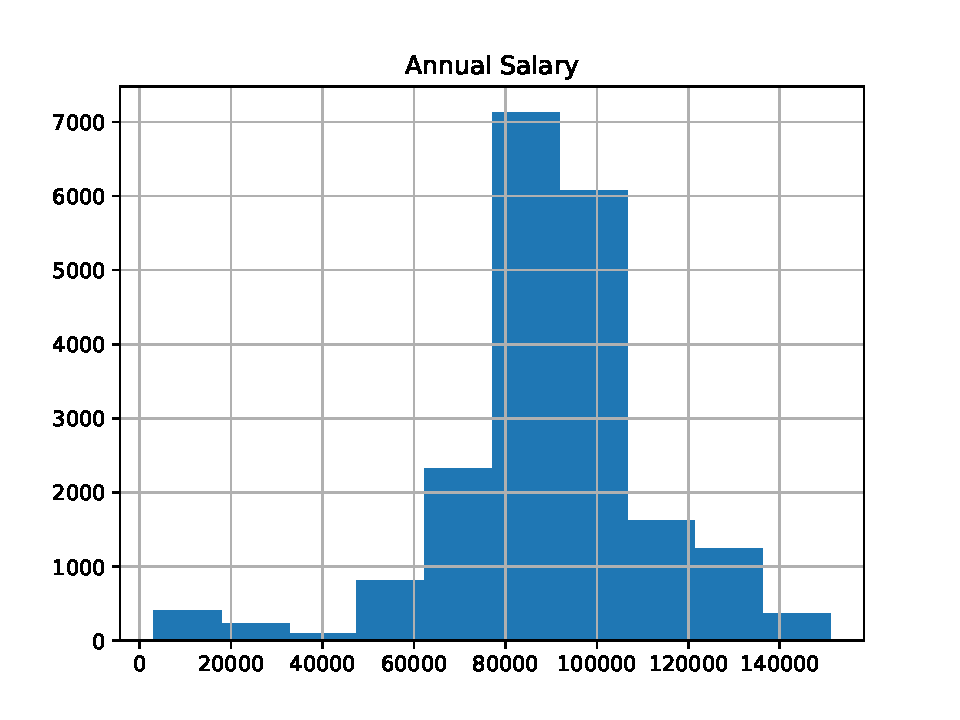
\includegraphics[width=0.75\textwidth]{figures/chicago_annual_salary_distribution.pdf}
\caption{Distribution of the \textrm{Annual Salary} values for the Chicago dataset.}
\label{fig:chicago_preprocessing1}
\end{figure}

Lastly, we decided to plot the \textit{probability mass function (PMF)} and the \textit{cumulative distribution function (CDF)} of male and female employees, for each \textit{Annual Salary} value. For the laymen, PMF gives the probability that a discrete variable -- \textit{Annual Salary} in our case -- is exactly equal to a specific value; while CDF is the probability of the variable to be less than or equal to a specific value. The comparison between Figure~\ref{fig:chicago_preprocessing2}(a) and Figure~\ref{fig:chicago_preprocessing2}(b) shows, once again, that women are more likely than men to earn less, and specifically to have an income in the range of [0,~40K] dollars per year.

\begin{figure}[t!]
\centering
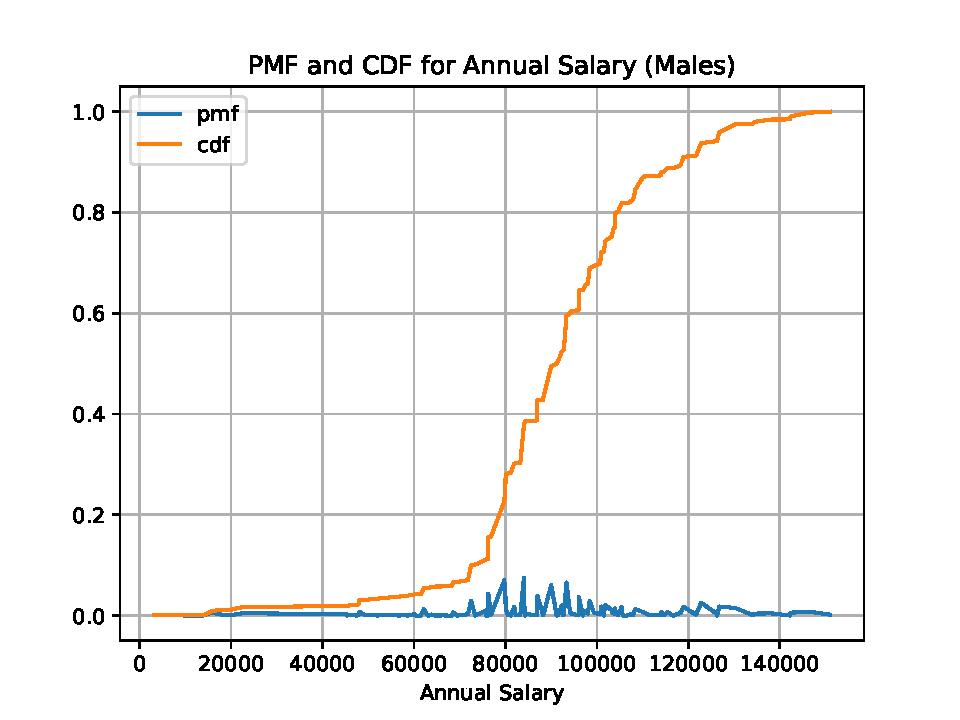
\includegraphics[width=0.75\textwidth]{figures/chicago_pmf_cdf_annual_salary_males.pdf}
\caption*{(a)}
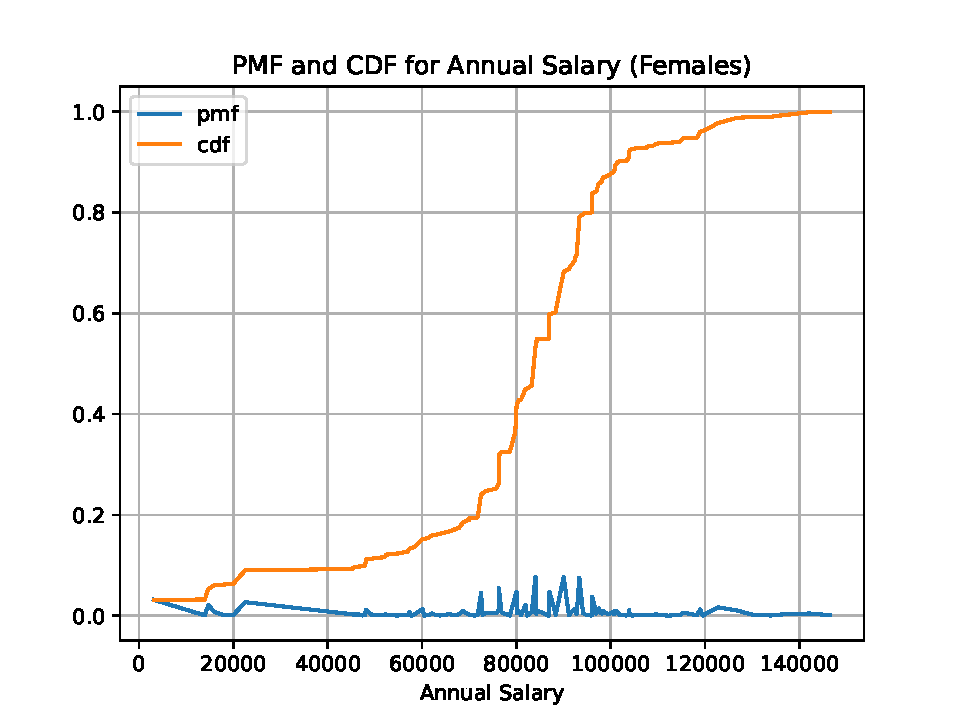
\includegraphics[width=0.75\textwidth]{figures/chicago_pmf_cdf_annual_salary_females.pdf}
\caption*{(b)}
\caption{Probability mass function and cumulative distribution function of male (a) and female (b) employees, for each \textrm{Annual Salary} value of the Chicago dataset.}
\label{fig:chicago_preprocessing2}
\end{figure}


\subsection{The ``Glassdoor Method''}
As already specified in Section~\ref{section:the_glassdoor_method}, the point of reference for this method is the report published by Glassdoor in 2017 with the aim of helping HR practitioners in analyzing the internal gender pay gap of their companies \cite{chamberlain2017analyze}. Although the report provides a step-by-step guide for the statistical software R, we decided to use Python for our analysis, in order to better integrate the results with the ones from the other tools.

The first step of the analysis, after cleaning up the data and loading them, consists in the creation of a couple of attributes useful for the statistical analysis: \textit{Log Annual Salary} and \textit{Male}. The former is simply the natural logarithm of the annual salary of the employee (i.e. the logarithm to the base of the mathematical constant \textit{e}, approximately equal to 2.71828), useful because it provides a simple interpretation of the regression results; the latter is a dummy indicator equal to 1 for males and 0 for females, which is the key variable of the analysis: if there is no gap, being male should not provide any advantage, and the coefficient of this variable in the regression should be equal to 0, otherwise its value would give us an estimate of the approximate percentage pay gap between men and women. It is worth to mention that the Glassdoor report also suggests to perform a discretization of age values of employees, grouping them into bins (25\(-\), 25--34, 35--44, 45--54, 55+), but our dataset does not contain any information about the age of the employees.

The report suggests to look at the data before proceeding with the regressions, and it recommends to print a ``summary table'' displaying the basic statistical information about the dataset. Figure~\ref{fig:chicago_glassdoor1}(a) shows the table related to the Chicago dataset, and it displays the variables \textit{Annual Salary}, \textit{Log Annual Salary}, and \textit{Male} sample size (count), arithmetic mean, minimum and maximum values, and standard deviation (i.e. a measure of the average amount of variability in the dataset -- calculated as the square root of the variance -- which tells, on average, how far each value lies from the mean).
Another useful visualization tool is the so called ``pivot table'', displayed in Figure~\ref{fig:chicago_glassdoor1}(b), which provides a high-level summary of the overall difference in pay between men and women by showing the arithmetic mean of the \textit{Annual Salary} attribute values for males and females, together with the number of observations (len) and the median values (i.e. the numeric values separating the higher half of the samples from the lower half). The pivot table is also useful to get a first estimate of the ``unadjusted'' pay gap: men on average are paid \$92,022.03 per year, while women on average earn \$79,790.83 per year -- an overall ``unadjusted'' pay gap of \$12,231.20 (13.3\% of male pay).
Lastly, since we are also interested in the ``adjusted'' pay gap, it is important to look at the average salaries of men and women employed in the different job titles. Figure~\ref{fig:chicago_glassdoor1}(c) shows the first 8 (out of 35) job titles in alphabetical order, displaying average salaries for men and women and sizes of the samples (i.e. number of men and women employed in the specific job title -- information relevant to the problem of representation).

\begin{figure}[t!]
\centering
\noindent\rule{\linewidth}{0.4pt}\par
%\resizebox{\linewidth}{!}{%
\scalebox{.9}{\BVerbatimInput{figures/chicago_glassdoor1a.txt}}
\caption*{(a)}
\noindent\rule{\linewidth}{0.4pt}\par
%\resizebox{\linewidth}{!}{%
\scalebox{.9}{\BVerbatimInput{figures/chicago_glassdoor1b.txt}}
\caption*{(b)}
\noindent\rule{\linewidth}{0.4pt}\par
%\resizebox{\linewidth}{!}{%
\scalebox{.9}{\BVerbatimInput{figures/chicago_glassdoor1c.txt}}
\caption*{(c)}
\noindent\rule{\linewidth}{0.4pt}
\caption{Summary table (a), pivot table (b) and average salaries of men and women employed in the different job titles (c) for the Chicago dataset.}
\label{fig:chicago_glassdoor1}
\end{figure}

In order to estimate the gender pay gap, the reference linear regression model, as mentioned in Section~\ref{section:the_glassdoor_method}, is: \[\mathit{Log Annual Salary}_i = \beta_1\textit{Male}_i + \beta_2\mathit{Controls}_i + \epsilon_i\]
The report recommends to execute three different linear regressions: the first with no controls at all, regressing salary only on the male-female gender dummy (and therefore calculating the approximate overall percentage pay gap between men and women -- the ``unadjusted'' pay gap); the second with the addition of variables related to employee characteristics like highest education, years of experience, and performance evaluation scores; the third including all the possible controls (and finally estimating the ``adjusted'' pay gap). Due to the lack of attributes, we performed only two linear regressions: the first with no controls and the second including \textit{Job Title}, \textit{Department}, and \textit{Status}.

\begin{figure}[t!]
\centering
\noindent\rule{\linewidth}{0.4pt}\par
%\resizebox{\linewidth}{!}{%
\scalebox{.9}{\BVerbatimInput{figures/chicago_glassdoor2.txt}}
\noindent\rule{\linewidth}{0.4pt}
\caption{Regression results for the Chicago dataset.}
\label{fig:chicago_glassdoor2}
\end{figure}

The results are shown in Figure~\ref{fig:chicago_glassdoor2}: a coefficient of 0.242 on the male-female dummy variable means there is approximately 24.2\% ``unadjusted'' pay gap (therefore, men on average earn 24.2\% more than women), but adding to the model all of the controls available in the data the coefficient value shrinks to 0.4\% and becomes no longer statistically significant. In this case, we say there is no evidence of a systematic gender pay gap on an ``adjusted'' basis, after controlling for observable differences between male and female workers, and the big discrepancy between the coefficient values is due to the overrepresentation of men in higher-paying roles and their underrepresentation in lower-paying jobs.


\subsection{FAIR-DB}
\label{section:chicago_fair-db}
FAIR-DB is a tool based on functional dependencies, as already described in Section~\ref{section:fair-db}, and it operates by following the workflow shown in Figure~\ref{fig:fair-db_framework}.
\begin{itemize}
\item \textbf{Data preparation and exploration}: this phase is mostly covered by Section~\ref{section:chicago_data_preprocessing}. In addition to the preprocessing techniques applied before, we had to deal with the \textbf{discretization} of \textit{Annual Salary} values, since numbers are not really useful in estimating correlations between attributes (functional dependencies may depend on really specific income values). We decided to create 2 interval levels (or bins) splitting \textit{Annual Salary} values in \(\leq\)~90K and >~90K and generating a new \textit{Annual Salary Bin} attribute to store this information, by following the approach presented in \cite{azzalini2021fair} by the authors of the tool. \textit{Annual Salary Bin} represents our \textbf{target attribute}, while \textit{Gender} is our \textbf{protected attribute}. The choice of 90K as threshold was made by looking at the \textit{Annual Salary} values distribution, shown in Figure~\ref{fig:chicago_preprocessing1}.

The histogram of Figure~\ref{fig:chicago_fair-db1} shows instead the distribution of the annual salary of employees over their \textit{Gender} attribute, and it is particularly useful because it provides a preliminary visual representation of the discrepancy between the number of male and female employees belonging to the same bin, highlighting the fact that, although the amount of people earning more than \$90,000 is larger, there are many more women in the least profitable group.

\begin{figure}[t!]
\centering
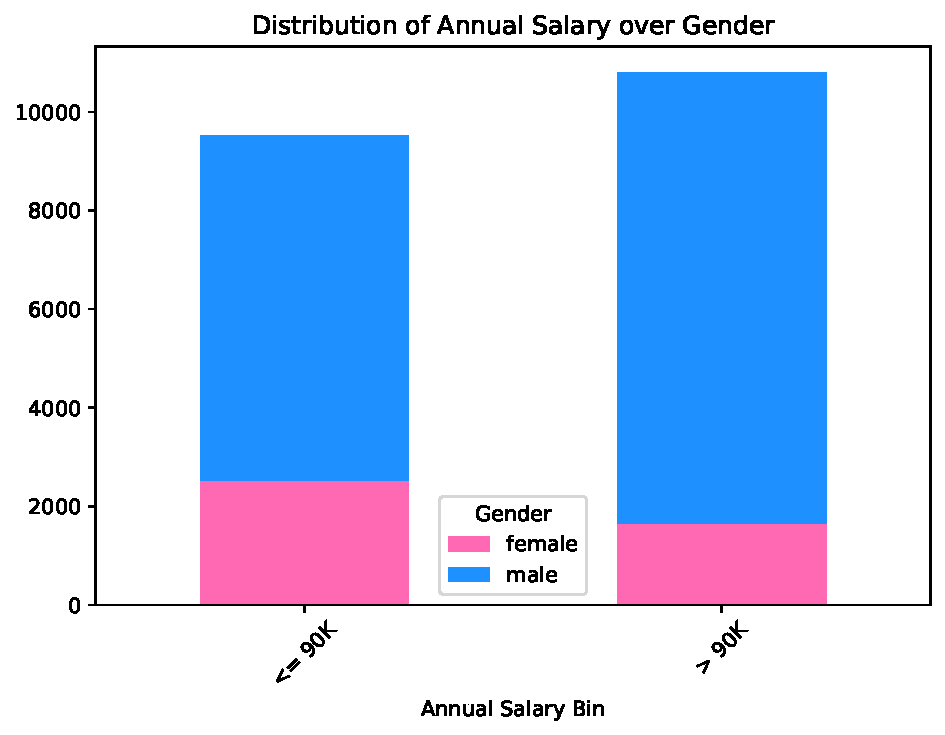
\includegraphics[width=0.75\textwidth]{figures/chicago_2bins_annual_salary_over_gender.pdf}
\caption{Distribution of the \textrm{Annual Salary} values for the Chicago dataset (2 bins).}
\label{fig:chicago_fair-db1}
\end{figure}

Lastly, we performed a new \textbf{data reduction} operation by removing from the dataset the attributes \textit{Name} and \textit{Annual Salary}, not relevant anymore for our analysis, since the tool will make use of the \textit{Annual Salary Bin} variable.
\item \textbf{ACFD Discovery and filtering}: as specified in Section~\ref{section:fair-db}, this phase makes use of the \textit{ACFD Discovery} algorithm, presented in \cite{rammelaere2018revisiting}. The authors of the algorithm made available a compute capsule on Code Ocean\footnote{Available at: \url{https://codeocean.com/capsule/6146641/tree}.}, which works basically as a Web-based application, allowing the user to upload a CSV file (in our case, we exported and uploaded the modified Chicago dataset), set the values of the required parameters (\textit{minimum support}, \textit{minimum confidence}, \textit{maximum antecedent size}), run the algorithm and download the results in the form of a text file. The software also allows the choice of different algorithm implementations to be used to extract the dependencies but, as reported in the documentation, the default option FD-First-DFS-dfs is generally the fastest and there are no particular reasons, apart from performances, to choose one implementation over another.

Since our dataset does not contain a large amount of attributes, we decided to keep \textit{maximum~antecedent~size}~=~2 (meaning that at most 2 variables will appear in the LHS of the computed rules).
For what concerns the confidence, its value is computed as the ratio between the frequency of the dependency over the frequency of the LHS of the rule, and therefore a \textit{minimum~confidence}~=~0.8 seemed to be a reasonable threshold, since the lower the parameter, the more dependencies are generated at each round increasing the computational complexity and making more difficult the subsequent choice of the most interesting ACFDs.
Finally, we had to deal with the choice of a proper minimum support, which is quite a delicate operation: if it is too high the risk is to lose information about small groups, if it is too low there could be too many dependencies to analyze. We set \textit{minimum~support}~=~100, because it is a reasonably low number if compared to the total number of tuples in the dataset and to the average amount of tuples for each \textit{Job Title} value (\(\frac{20,309}{35} \simeq 580\)).

The text file generated by \textit{ACFD Discovery}, containing 714 rules, has to be filtered, since the dependencies detected may not involve the protected attribute or the target attribute; there could also be dependencies in which some attribute values are not specified. The authors of \cite{azzalini2021fair} did not use the compute capsule of \textit{ACFD Discovery}, and therefore were able to run the algorithm with an additional parameter, in order to discard the rules not containing the target attribute and its value. We balanced the gap by importing the text file, parsing it in order to extract every rule, and doing the same filtering operation a posteriori of \textit{ACFD Discovery}. This operation resulted in a reduction in the number of dependencies from 714 to 145.

FAIR-DB then proceeds in filtering the rules by following 4 steps:
\begin{itemize}
\item[1.] For each dependency, the LHS is separated from the RHS, and from both antecedent and consequent every couple ``attribute - value'' is stored.
\item[2.] For each rule, every couple ``attribute - value'' is checked, and dependencies with missing values are discarded (being AFDs but not ACFDs).
\item[3.] A dictionary (that is, an unordered and indexed data structure similar to a list) of the remaining ACFDs is generated. It is made of two fields: `lhs' and `rhs', and each field contains a list of one or more couples ``attribute - value''.
\item[4.] Since each rule of the dictionary contains the target attribute but not necessarily any protected attribute, the dependencies are furtherly parsed in order to satisfy both the criteria.
\end{itemize}

For the Chicago dataset, the filtering operation resulted in a reduction in the number of dependencies from 145 to 49. For each rule, the metrics \textit{support}, \textit{confidence}, \textit{difference} and \textit{p-Difference}, already introduced in Section~\ref{section:evaluation_metrics} and Section~\ref{section:fair-db}, are computed, and the first occurrences are displayed in the form of a table, as shown in Figure~\ref{fig:chicago_fair-db2}.

\begin{figure}[t!]
\centering
\noindent\rule{\linewidth}{0.4pt}\par
%\resizebox{\linewidth}{!}{%
\scalebox{.9}{\BVerbatimInput{figures/chicago_fair-db2.txt}}
\noindent\rule{\linewidth}{0.4pt}
\caption{First 5 filtered dependencies with their metrics for the Chicago dataset (2 bins). NaN (Not a Number) means that the p-Difference has not been computed for the specific rule, since the protected attribute is not in the antecedent.}
\label{fig:chicago_fair-db2}
\end{figure}

\item \textbf{ACFD selection}: in this phase FAIR-DB selects, among the filtered rules, the most ``unethical'' according to the group fairness criterion, by looking at the computed metrics. It is worth to briefly recap the meanings behind the measures:
\begin{itemize}
\item \textbf{Support}: it expresses the percentage of records in the dataset that verifies the dependency -- the higher the value, the more tuples are involved.
\item \textbf{Confidence}: it shows how frequently the dependency is verified knowing that the antecedent is verified -- the higher the value, the less approximate is the dependency.
\item \textbf{Difference}: it indicates how much a dependency is ``unethical'' -- the higher the value, the more unfair is the dependency.
\item \textbf{p-Difference}: it indicates how much the dependency shows bias paying attention to the specific value of a protected attribute -- the higher the value, the more the rule is discriminatory with respect to the specific protected attribute value.
\end{itemize}

The selection of the most relevant rules takes place automatically, since the algorithm only keeps the dependencies with a difference parameter value higher than a minimum threshold imposed by the user. We decided to set \textit{minimum~difference}~=~0.02, in order to keep the majority of the unfair dependencies, avoiding unintentionally ignoring some rules that could instead be relevant for us. This operation resulted in a reduction in the number of dependencies from 49 to 10.

After that, the algorithm performs what the authors call \textbf{ACFD completion}. Given the selected ACFDs, the framework computes all the possible combinations for each rule over the protected attributes and the target attribute (performing a Cartesian product between the attribute values). Taking as an example ACFD n.0 of Figure~\ref{fig:chicago_fair-db2}: \[\mathit{Annual Salary Bin} = \mlq > 90K \mrq \rightarrow \mathit{Gender} = \mlq \mathrm{male} \mrq\] we identify \textit{Annual Salary Bin} as target attribute, whose possible values are \(\leq\)~90K and >~90K, and \textit{Gender} as protected attribute, whose possible values are male and female. Therefore, the possible combinations for the rule are:
\begingroup\belowdisplayskip=\belowdisplayshortskip
\[\mathit{Annual Salary Bin} = \mlq > 90K \mrq \rightarrow \mathit{Gender} = \mlq \mathrm{male} \mrq\]\endgroup
\[\mathit{Annual Salary Bin} = \mlq \leq 90K \mrq \rightarrow \mathit{Gender} = \mlq \mathrm{male} \mrq\]
\[\mathit{Annual Salary Bin} = \mlq > 90K \mrq \rightarrow \mathit{Gender} = \mlq \mathrm{female} \mrq\]
\[\mathit{Annual Salary Bin} = \mlq \leq 90K \mrq \rightarrow \mathit{Gender} = \mlq \mathrm{female} \mrq\]
For each newly generated dependency, the evaluation metrics are computed, and a new automatic selection is performed, by keeping the rules with difference greater than the respective minimum threshold. ACFD completion basically allows the user to study all the domain of the protected attributes and of the target class, and the combination computation brings to the surface also small groups that could not be studied otherwise. This operation, for the Chicago dataset, generated 36 dependencies (including the original 10), 18 of which have a difference above the threshold.
\item \textbf{ACFD ranking}: the dependencies are ranked in descending order of support, difference, or mean, according to the user choice. As already mentioned in Section~\ref{section:fair-db}, the support option highlights the pervasiveness of the rules, the difference highlights their unethical aspect, and the mean represents the best trade-off between difference and support. Because of that, we decided to adopt the mean as ordering criterion. The resulting table is finally printed, and Figure~\ref{fig:chicago_fair-db3} shows the first 5 dependencies (the others are displayed to the user but are omitted here for the sake of brevity).

\begin{figure}[t!]
\centering
\noindent\rule{\linewidth}{0.4pt}\par
%\resizebox{\linewidth}{!}{%
\scalebox{.9}{\BVerbatimInput{figures/chicago_fair-db3.txt}}
\noindent\rule{\linewidth}{0.4pt}
\caption{First 5 selected and ranked dependencies with their metrics for the Chicago dataset (2 bins).}
\label{fig:chicago_fair-db3}
\end{figure}

\item \textbf{ACFD user selection and scoring}: this last phase requires interaction from the user, who has to select \(N\) interesting dependencies among the ones previously ranked. The system then computes a final scoring outline based on 3 measures:
\begin{itemize}
\item \textbf{Cumulative support}: percentage of tuples of the dataset involved by the selected ACFDs -- the higher the value, the more tuples are involved.
\item \textbf{Difference mean}: arithmetic mean of all the `Difference' columns of the selected ACFDs. It indicates how much the dataset is ethical according to the chosen rules -- the higher the value, the more unfair is the dataset.
\item \textbf{Protected attribute difference mean}: for each protected attribute, arithmetic mean of the p-Difference measure over all the selected ACFDs. It indicates how much the dataset is ethical over the protected attribute according to the chosen rules -- the higher the value, the more the dataset is discriminatory with respect to the specific protected attribute.
\end{itemize}

For our research, we selected all the dependencies in which the target attribute appears in the RHS of the rule (\(N\) = 6 out of 18). This choice is due to the fact that the authors did not specify any criteria or suggestion for the manual selection of the rules, and the algorithm does not consider rules in which the protected attribute appears in the RHS as biased with respect to the protected attribute itself, in fact, as can be noticed in Figure~\ref{fig:chicago_fair-db3}, rules in which the protected attribute is in the RHS have a NaN (not computed) p-Difference value, while the same statistical measure is never NaN when the protected attribute is in the LHS. Other dependencies, in which both target attribute and protected attribute appear in the RHS, are not particularly relevant for us, precisely because none of our variables of interest is functionally dependent upon the other. We will furtherly discuss about the impact of this choice in Section~\ref{section:XYZ}. The chosen ACFDs, together with the final scores, are displayed in Figure~\ref{fig:chicago_fair-db4}.

\begin{figure}[t!]
\centering
\noindent\rule{\linewidth}{0.4pt}\par
%\resizebox{\linewidth}{!}{%
\scalebox{.9}{\BVerbatimInput{figures/chicago_fair-db4.txt}}
\noindent\rule{\linewidth}{0.4pt}
\caption{Final selected rules and scores for the Chicago dataset (2 bins).}
\label{fig:chicago_fair-db4}
\end{figure}
\end{itemize}

Among the chosen dependencies, we can detect a correspondency between rule 7 and rule 4: women paid on a hourly basis tend to earn less than \$90K, while men paid on a hourly basis tend to earn more than \$90K. These rules are the ones with the highest support (respectively 0.03 and 0.07), and rule 7 is the one with the highest difference value (0.24).

Even though the support is very low -- and therefore not many tuples out of the total are involved -- it is important to point out that rules 27 and 24 suggest a discriminatory behavior in the subgroup of the AVIATION department, while rules 29 and 30 show that, for what concerns the OEMC department, men seem to be less paid than women. The main reasons for these behaviors are a disproportion, in favor of male employees, in the number of men and women employed in the AVIATION department, and, on the contrary, a disproportion, in favor of female employees, in the number of men and women employed in the OEMC one. Disproportions can cause these situations when, within a dataset and for a specific job title, there are some tuples with income above the threshold for both men and women but, for one of the two genders, the proportion of these tuples with respect to the total is very small compared to the other one. In this dataset, for example, for the OEMC department, the number of male employees earning more than \$90K is 9 (out of 147 men employed in OEMC), while the number of female employees earning more than \$90K is 73 (out of 414 women employed in OEMC). Although on average both men and women earn less than \$90K, the disproportion makes the algorithm perceive a discriminatory behavior towards male employees.

As for the scoring measures, a cumulative support of 0.114 means that the 11.4\% of the dataset is ``problematic'' (2,310 tuples out of 20,309), while difference mean and gender difference mean (equal because in our dataset \textit{Gender} is the only protected attribute) have a value of 0.094 because of the gap between the difference metric values of the selected ACFDs (above 0.1 for rule 27, above 0.2 for rule 7, below 0.1 for the other rules).

To conclude, we can say that the dataset seems to be quite fair with respect to the group fairness criterion, that is the one on which the tool is based, but more than 10\% of the tuples show bias. Furthermore, the representation problem is not taken into account, and therefore the tendency of women to be employed in less profitable jobs than men, displayed in Figure~\ref{fig:chicago_preprocessing2} and Figure~\ref{fig:chicago_fair-db2}, is ignored.


\subsection{Ranking Facts}
As specified in Section~\ref{section:ranking_facts}, Ranking Facts is primarily meant to be a Web-based application with the aim of discovering fairness in a dataset by making use of ranking and providing to the user a collection of visual widgets. However, because of the size of our dataset, we could not use the tool in the form of a Web-based application, and we had to opt for the notebook version.

Before importing the dataset, we had to deal with a further \textbf{data transformation} process, in which we converted our categorical attributes (\textit{Status}, \textit{Job Title}, \textit{Department}, \textit{Salary or Hourly}) into numerical ones, since the tool can perform ranking only over them. A value of F for the \textit{Status} attribute was therefore converted to 1, while P was converted to 0. The same holds for \textit{Salary or Hourly} (Salary = 1, Hourly = 0), while for \textit{Job Title} and \textit{Department} numbers from 0 to 35 and from 0 to 20 respectively substited the original categorical values.

Once imported the dataset, the tool initially plots the distribution of some attributes specified by the user (in our case, we decided to plot the distributions of the \textit{Annual Salary} and \textit{Gender} values). While the related distribution graphs are not particularly meaningful, the heatmap generated subsequently provides us with some preliminary information about the attribute correlations. As Figure~\ref{fig:chicago_rankingfacts1} shows, there seems to be a significant correlation between \textit{Job Title} and \textit{Department}, but mostly important between \textit{Status} and \textit{Annual Salary}, \textit{Status} and \textit{Salary or Hourly}, and finally \textit{Annual Salary} and \textit{Salary or Hourly}, highlighting the fact that hourly paid and part-time employees earn generally less than salary paid and full-time employees, and most of the part-time workers are also being paid on a hourly basis.

\begin{figure}[t!]
\centering
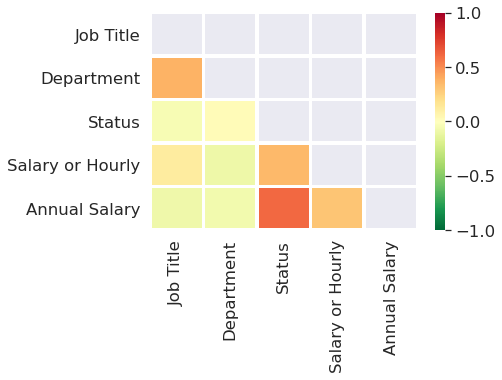
\includegraphics[width=0.7\textwidth]{figures/chicago_rankingfacts1.png}
\caption{Heatmap showing attribute correlations for the Chicago dataset.}
\label{fig:chicago_rankingfacts1}
\end{figure}

The tool then requires the user to specify some attributes to be used for the ranking, together with their weights. The reference formula is: \[f(x) = w_1 \times \mathit{Attribute}_1(x) + \ldots + w_n \times \mathit{Attribute}_n(x)\]
In our case, the attributes used are \textit{Job Title}, \textit{Department}, \textit{Status}, \textit{Salary or Hourly}, and \textit{Annual Salary}, because they are numerical and none of them is a protected variable. By following the examples provided by the authors of the tool, we decided to set the weights all equal to 1, giving the same importance to each attribute.

By following the widget description list provided in Section~\ref{section:ranking_facts}, we will now summarize our results.
\begin{itemize}
\item \textbf{Recipe} and \textbf{Ingredients}: the notebook version of the tool unfortunately does not provide any visual representation. As for the recipe, a couple of summary tables display some statistical measures (median, mean, minimum and maximum value) for the 4 attributes used in the ranking, respectively for the top-10 one and overall. These tables are not particularly useful, and neither is the information related to the ingredients, which tells us that the importance of each attribute used for the ranking is effectively equal to 1.
\item \textbf{Stability}: this parameter explains whether the ranking methodology is robust on the specific dataset in use. Since an unstable ranking is one where slight changes to the data or to the methodology could lead to a significant change in the output, the label reports a stability score, as a single number that indicates the extent of the change required for the ranking to change. The stability of the ranking is quantified as the slope of the line that is fit to the score distribution, at the top-10 and overall. A score distribution is unstable if scores of items in adjacent ranks are close to each other (\(|\mathit{slope}| \leq 0.25\)), and so a very small change in scores will lead to a change in the ranking. The ranking used to analyze the Chicago dataset resulted to be stable at top-10 (stability at 0.39) but unstable overall (stability at 0.0), and the score distribution is displayed in Figure~\ref{fig:chicago_rankingfacts2}.

\begin{figure}[t!]
\centering
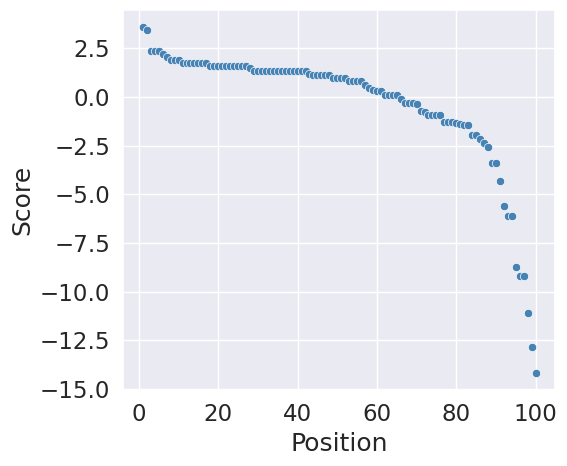
\includegraphics[width=0.7\textwidth]{figures/chicago_rankingfacts2.png}
\caption{Score distribution of the ranking for the Chicago dataset.}
\label{fig:chicago_rankingfacts2}
\end{figure}

\item \textbf{Fairness}: it quantifies whether the ranked output exhibits statistical parity (group fairness) with respect to one or more protected attributes. The fairness measures adopted are all statistical tests in which the null hypothesis is that the ranking process is fair for the protected group, and whether a result is fair is determined by the computed \(p\)-value (a ranking is considered unfair when the \(p\)-value of the corresponding statistical test falls below 0.05).
\begin{itemize}
\item \textbf{FA*IR}: the ranking resulted to be \textit{fair for males}, with an approximate \(p\)-value of 0.84, and \textit{unfair for females}, with an approximate \(p\)-value of 0.16.
\item \textbf{Proportion}: the ranking resulted to be \textit{fair for males}, with an approximate \(p\)-value of 0.97, and \textit{fair for females}, with an approximate \(p\)-value of 0.35.
\item \textbf{Pairwise}: the ranking resulted to be \textit{fair for males}, with an approximate \(p\)-value of 0.31, and \textit{fair for females}, with an approximate \(p\)-value of 0.65.
\end{itemize}
The results seem to be oriented towards a fair dataset, even though the FA*IR measure reported the presence of bias in favor of men.
\item \textbf{Diversity}: it shows diversity with respect to a set of demographic categories of individuals, or a set of categorical attributes of other kinds of items, by displaying the proportion of each category in the top-10 ranked list and overall. Figure~\ref{fig:chicago_rankingfacts3} shows the predominancy of the male group over the female one, especially in the top-10 of the ranking, highlighting again a problem of gender representation.

\begin{figure}[t!]
\centering
\begin{minipage}{0.45\textwidth}
\centering
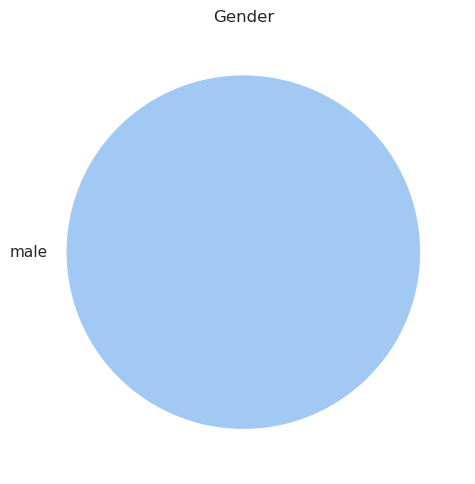
\includegraphics[width=\textwidth]{figures/chicago_rankingfacts3a.png}
\caption*{(a)}
\end{minipage}
\begin{minipage}{0.45\textwidth}
\centering
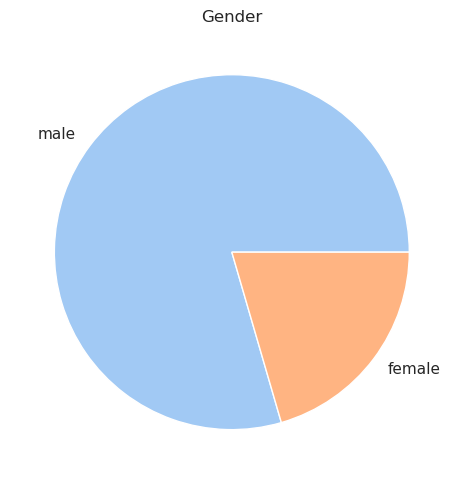
\includegraphics[width=\textwidth]{figures/chicago_rankingfacts3b.png}
\caption*{(b)}
\end{minipage}
\caption{\textrm{Gender} diversity widget for the top-10 (a) and overall (b) rankings of the Chicago dataset.}
\label{fig:chicago_rankingfacts3}
\end{figure}

\end{itemize}


\section{Case Study 2: San Francisco}
\subsection{Dataset Description}
The \textbf{San Francisco} dataset we considered includes 357,407 tuples and is made up of 10 attributes, briefly described as follows:
\begin{itemize}
\item \textit{Employee Name}: full name of the employee in the form of ``Name Surname''.
\item \textit{Job Title}: categorical variable representing the job title of the employee (e.g. Firefighter). There are 2306 distinct values.
\item \textit{Base Pay}: numerical variable describing the annual regular pay for the employee.
\item \textit{Overtime Pay}: numerical variable describing the annual overtime pay for the employee.
\item \textit{Other Pay}: numerical variable describing other annual pay components for the employee.
\item \textit{Benefits}: numerical variable describing the amount of annual benefits for the employee.
\item \textit{Total Pay}: numerical variable describing the total annual salary of the employee, benefits excluded (\textit{Base Pay} + \textit{Overtime Pay} + \textit{Other Pay}).
\item \textit{Total Pay + Benefits}: numerical variable describing the total annual salary of the employee, benefits included (\textit{Base Pay} + \textit{Overtime Pay} + \textit{Other Pay} + \textit{Benefits}).
\item \textit{Year}: numerical variable representing the year of reference (the dataset contains data related to the years 2011 to 2019).
\item \textit{Status}: binary categorical variable describing whether the employee is employed full-time (FT) or part-time (PT).
\end{itemize}


\subsection{Data Preprocessing}
\label{section:san_francisco_data_preprocessing}
As for the Chicago case, we operated some \textbf{data transformation} processes on the attributes of the San Francisco dataset. Specifically, the columns \textit{Employee Name} and \textit{Total Pay} were renamed respectively to \textit{Name} and \textit{Annual Salary}, and the attribute values for \textit{Status} were transformed from FT and PT to simply F and P, in order to keep the algorithm used for the subsequent bias analysis as simple as possible and have a consistent structure across the datasets in use. We also operated a significant \textbf{data cleaning}, by filtering the tuples on the \textit{Year} attribute, and keeping only the ones with \textit{Year} = 2019, since they are the most recent and we want to avoid redundant data across multiple years. This operation resulted in a reduction in the number of tuples from 357,407 to 44,525.

Again, since the original dataset does not contain any gender-related information, we relied on \texttt{gender-guesser} to infer the gender of the employees from their \textit{First Name}, by splitting the \textit{Name} attribute and saving the results in a newly generated \textit{Gender} attribute. We obtained (out of the total of 44,525 tuples):
\begin{itemize}
\item unknown: 5,096 values.
\item andy: 1,975 values.
\item male: 20,636 values.
\item female: 14,283 values.
\item mostly\_male: 1,153 values.
\item mostly\_female: 1,382 values.
\end{itemize}
We then removed, as we did for the Chicago dataset, tuples related to unknown and androgynous names, and we assumed mostly male names to be effectively related to males and mostly female names to be effectively related to females, and therefore we got 21,789 male values and 15,665 female values as a result of this \textbf{data cleaning} process.

We also operated \textbf{data reduction} by removing the \textit{Base Pay}, \textit{Overtime Pay}, \textit{Other Pay}, \textit{Benefits}, \textit{Total Pay \& Benefits}, \textit{Year}, and \textit{First Name} columns, since the information concerning the year became no longer useful and for the purpose of this research we are only interested in the total annual salary of employees.

Finally, we performed a last \textbf{data cleaning} process by removing job titles with less than 100 occurrences.

Our final preprocessed dataset includes 22,996 tuples, of which 13,688 males and 9,308 females, and with 81 distinct \textit{Job Title} values.

Figure~\ref{fig:san_francisco_preprocessing1} shows the \textit{Annual Salary} values distribution, from which we can observe that the lowest paid jobs are the most common, and the largest group of employees earns less than \$50,000. This is due to the fact that, in comparison with the Chicago dataset, the San Francisco one contains many more part-time employees (9,308 out of 22,996 tuples for San Francisco, 639 out of 20,309 tuples for Chicago), and many job titles are monopolized or nearly monopolized by them, such as Pool Lifeguard, School Crossing Guard, or Recreation Leader.

\begin{figure}[t!]
\centering
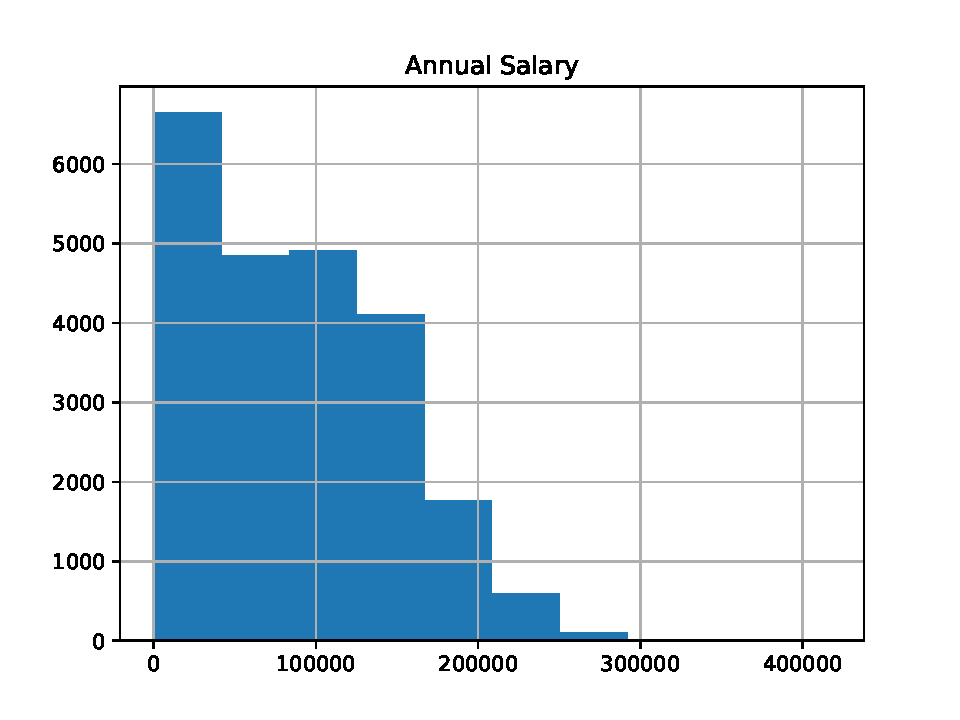
\includegraphics[width=0.75\textwidth]{figures/san_francisco_annual_salary_distribution.pdf}
\caption{Distribution of the \textrm{Annual Salary} values for the San Francisco dataset.}
\label{fig:san_francisco_preprocessing1}
\end{figure}

Lastly, Figure~\ref{fig:chicago_preprocessing2}(a) and Figure~\ref{fig:chicago_preprocessing2}(b) display probability mass function (PMF) and cumulative distribution function (CDF) of male and female employees, for each \textit{Annual Salary} value. PMF is not particularly relevant in this case because of its constant value, but CDF shows that the higher-paying jobs are done almost exclusively by men (even though the graphs look quite similar, the x-axis scale is different and it extends up to \$400,000 only on the male one). Again, women are more likely than men to earn less, since the curve on the female graph increases more rapidly compared to the male one (representing a higher probability to have a lower income).

\begin{figure}[t!]
\centering
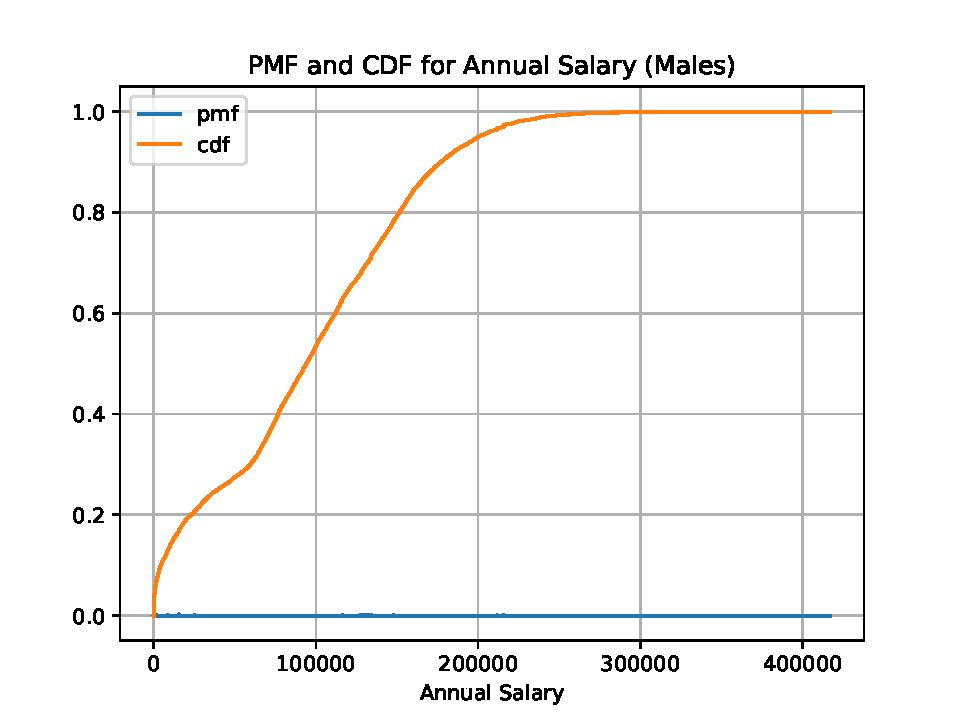
\includegraphics[width=0.75\textwidth]{figures/san_francisco_pmf_cdf_annual_salary_males.pdf}
\caption*{(a)}
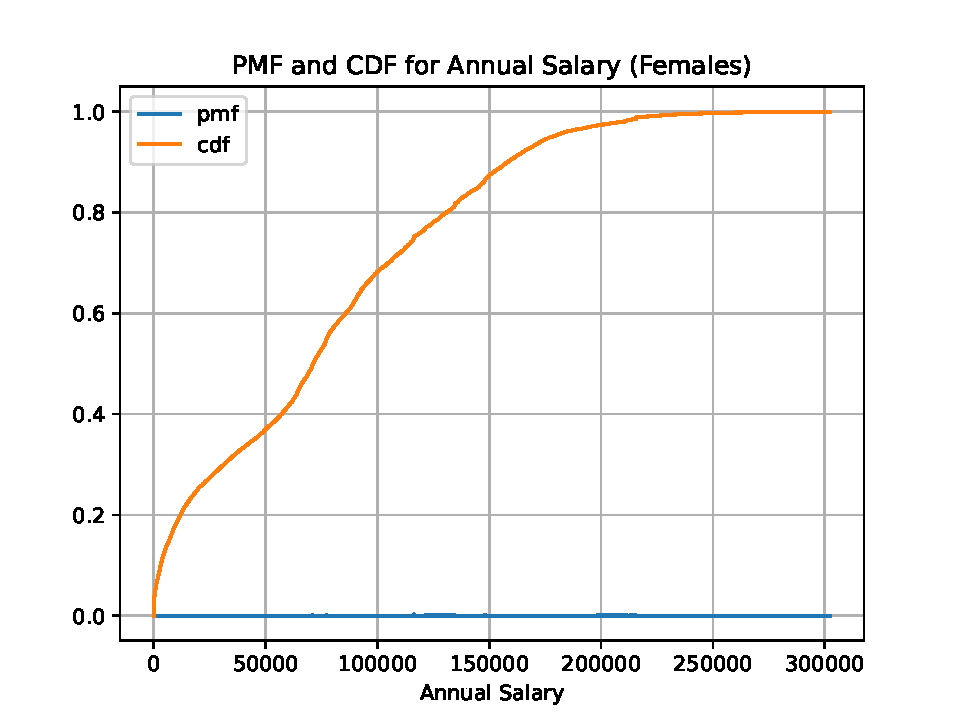
\includegraphics[width=0.75\textwidth]{figures/san_francisco_pmf_cdf_annual_salary_females.pdf}
\caption*{(b)}
\caption{Probability mass function and cumulative distribution function of male (a) and female (b) employees, for each \textrm{Annual Salary} value of the San Francisco dataset.}
\label{fig:san_francisco_preprocessing2}
\end{figure}


\subsection{The ``Glassdoor Method''}
As for the Chicago case, we started by creating the \textit{Log Annual Salary} and \textit{Male} attributes, useful for the statistical analysis. After that, we proceeded in printing the summary and pivot tables, shown respectively in Figure~\ref{fig:san_francisco_glassdoor1}(a) and Figure~\ref{fig:san_francisco_glassdoor1}(b). Since men on average are paid \$94,370.73 per year, while women on average earn \$75,841.50 per year, we got a first estimate of the overall ``unadjusted'' pay gap of \$18,529.23 (19.6\% of male pay). Figure~\ref{fig:san_francisco_glassdoor1}(c) shows the first 8 (out of 81) job titles in alphabetical order, displaying average salaries for men and women and sizes of the samples.

\begin{figure}[t!]
\centering
\noindent\rule{\linewidth}{0.4pt}\par
%\resizebox{\linewidth}{!}{%
\scalebox{.9}{\BVerbatimInput{figures/san_francisco_glassdoor1a.txt}}
\caption*{(a)}
\noindent\rule{\linewidth}{0.4pt}\par
%\resizebox{\linewidth}{!}{%
\scalebox{.9}{\BVerbatimInput{figures/san_francisco_glassdoor1b.txt}}
\caption*{(b)}
\noindent\rule{\linewidth}{0.4pt}\par
%\resizebox{\linewidth}{!}{%
\scalebox{.9}{\BVerbatimInput{figures/san_francisco_glassdoor1c.txt}}
\caption*{(c)}
\noindent\rule{\linewidth}{0.4pt}
\caption{Summary table (a), pivot table (b) and average salaries of men and women employed in the different job titles (c) for the San Francisco dataset.}
\label{fig:san_francisco_glassdoor1}
\end{figure}

Again, because of the lack of attributes, we could perform only two linear regressions: the first with no controls and the second including \textit{Job Title} and \textit{Status}.

\begin{figure}[t!]
\centering
\noindent\rule{\linewidth}{0.4pt}\par
%\resizebox{\linewidth}{!}{%
\scalebox{.9}{\BVerbatimInput{figures/san_francisco_glassdoor2.txt}}
\noindent\rule{\linewidth}{0.4pt}
\caption{Regression results for the San Francisco dataset.}
\label{fig:san_francisco_glassdoor2}
\end{figure}

The results are shown in Figure~\ref{fig:san_francisco_glassdoor2}: a coefficient of 0.304 on the male-female dummy variable means there is approximately 30.4\% ``unadjusted'' pay gap (therefore, men on average earn 30.4\% more than women), but adding to the model all of the controls available in the data the coefficient value shrinks to \(-\)0.5\% and becomes no longer statistically significant. We can conclude that also in this case there is no evidence of a systematic gender pay gap on an ``adjusted'' basis, after controlling for observable differences between male and female workers, and again the big discrepancy between the coefficient values is due to the overrepresentation of men in higher-paying roles and their underrepresentation in lower-paying jobs.


\subsection{FAIR-DB}
\begin{itemize}
\item \textbf{Data preparation and exploration}: in addition to the preprocessing techniques applied in Section~\ref{section:san_francisco_data_preprocessing}, we had once again to deal with the \textbf{discretization} of \textit{Annual Salary} values and the creation of a new \textit{Annual Salary Bin} attribute. By looking at the graph displayed in Figure~\ref{fig:san_francisco_preprocessing1}, we decided to keep 90K as threshold value, and therefore to use the same bins (\(\leq\)~90K and >~90K) used for the Chicago case.

The histogram of Figure~\ref{fig:san_francisco_fair-db1} shows the distribution of the annual salary of employees over their \textit{Gender} attribute. As we can notice, although the number of male and female employees belonging to the \(\leq\)~90K bin is comparable, almost \(\frac{2}{3}\) of the employees belonging to the >~90K bin are men.

\begin{figure}[t!]
\centering
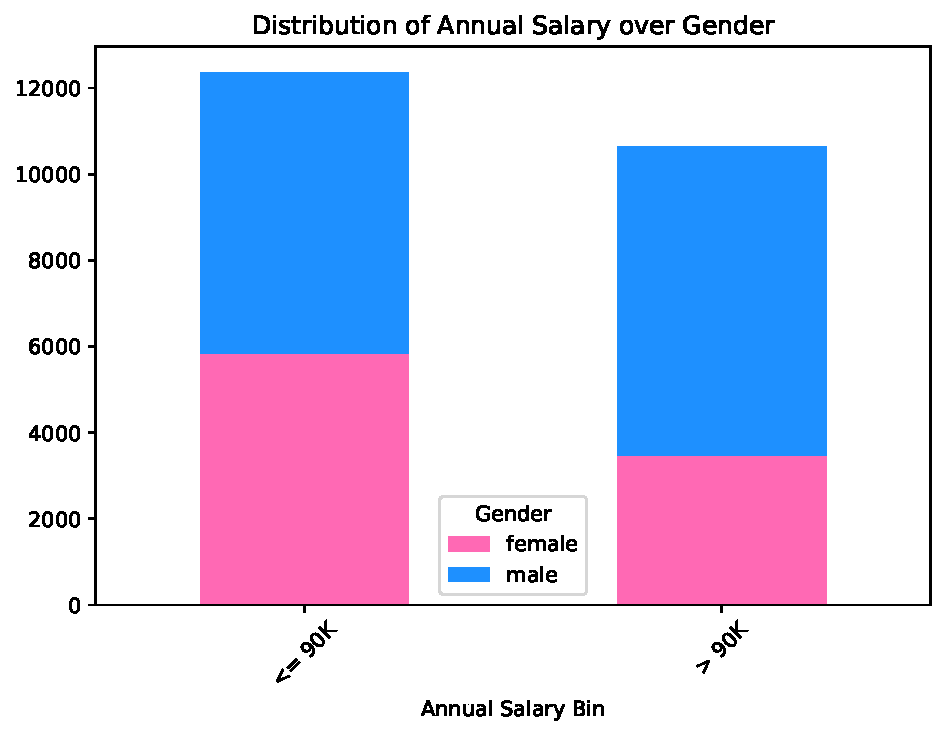
\includegraphics[width=0.75\textwidth]{figures/san_francisco_2bins_annual_salary_over_gender.pdf}
\caption{Distribution of the \textrm{Annual Salary} values for the San Francisco dataset (2 bins).}
\label{fig:san_francisco_fair-db1}
\end{figure}

Lastly, we performed a new \textbf{data reduction} operation by removing from the dataset the attributes \textit{Name} and \textit{Annual Salary}, since the tool will make use of the \textit{Annual Salary Bin} variable.
\item \textbf{ACFD Discovery and filtering}: we used the compute capsule of the \textit{ACFD Discovery} algorithm as we did for the Chicago case, and we decided to keep the same parameter values: \textit{maximum~antecedent~size}~=~2 because the dataset does not contain many attributes, \textit{minimum~confidence}~=~0.8 to generate not too high a number of dependencies, and \textit{minimum~support}~=~100 because it is a reasonably low number if compared to the total number of tuples in the dataset and to the average amount of tuples for each \textit{Job Title} value (\(\frac{22,996}{81} \simeq 284\)).

The text file generated by \textit{ACFD Discovery}, containing 586 dependencies, was then imported, parsed, and filtered in order to discard the rules not containing the target attribute and its value. This operation resulted in a reduction in the number of dependencies from 586 to 220. The automatic filtering operations performed by FAIR-DB further reduced this number from 220 to 61.
\item \textbf{ACFD selection}: as for the previous phase, we decided to maintain the same value for the only parameter required by ACFD selection, and therefore we set \textit{minimum~difference}~=~0.02 in order to keep the majority of the unfair dependencies. The first automatic selection resulted in a reduction in the number of dependencies from 61 to 10. The subsequent ACFD completion and further selection generated 36 dependencies (including the original 10), 16 of which have a difference above the threshold.
\item \textbf{ACFD ranking}: Figure~\ref{fig:san_francisco_fair-db2} shows the first 5 dependencies, ranked according to the mean (the others are displayed to the user but are omitted here for the sake of brevity).

\begin{figure}[t!]
\centering
\noindent\rule{\linewidth}{0.4pt}\par
%\resizebox{\linewidth}{!}{%
\scalebox{.9}{\BVerbatimInput{figures/san_francisco_fair-db2.txt}}
\noindent\rule{\linewidth}{0.4pt}
\caption{First 5 selected and ranked dependencies with their metrics for the San Francisco dataset (2 bins).}
\label{fig:san_francisco_fair-db2}
\end{figure}

\item \textbf{ACFD user selection and scoring}: for the reasons already specified in Section~\ref{section:chicago_fair-db}, we selected all the dependencies in which the target attribute appears in the RHS of the rule (\(N\) = 10 out of 16). The chosen ACFDs, together with the final scores, are displayed in Figure~\ref{fig:san_francisco_fair-db3}.

\begin{figure}[t!]
\centering
\noindent\rule{\linewidth}{0.4pt}\par
%\resizebox{\linewidth}{!}{%
\scalebox{.9}{\BVerbatimInput{figures/san_francisco_fair-db3.txt}}
\noindent\rule{\linewidth}{0.4pt}
\caption{Final selected rules and scores for the San Francisco dataset (2 bins).}
\label{fig:san_francisco_fair-db3}
\end{figure}
\end{itemize}

Among the chosen dependencies, we can detect a correspondency between rule 1 and rule 2: apparently, female part-time workers tend to earn more than \$90K, while male part-time workers tend to earn less than \$90K. These rules are the ones with the highest support (respectively 0.19 and 0.02). By looking at the average salaries of men and women employed in the different job titles, we found a few reasons for this behavior: first of all, in general there are many more part-time female employees out of the total number of women in the dataset, in comparison to men (4,162 out of 9,308 tuples for women, 4,606 out of 13,688 tuples for men); secondly, there are some typically masculine jobs (e.g. Automotive Mechanic, Electronic Maintenance Tech, Stationary Engineer) in which just a few women are employed, as full-time workers, while men are much more numerous and spredead among full-time and part-time positions, and for these jobs the part-time income is on average lower than the threshold. On the contrary, there are some typically feminine jobs (e.g. Medical Evaluations Assistant, Nurse Practitioner, Registered Nurse) in which just a few men are employed, as full-time workers, while women are much more numerous and spredead among full-time and part-time positions, and for these jobs the part-time income is on average higher than the threshold.

Even though the support is very low -- and therefore not many tuples out of the total are involved -- it is important to point out that rules 19 and 16 suggest a discriminatory behavior in the subgroup of the Assoc Engineer job title in favor of men (with the highest difference value for rule 19), and the same holds for rules 23 and 20 in the subgroup of assistant engineers. The main reason for these behaviors is a disproportion, in favor of male employees, in the number of men and women employed in these profitable professions.

Although the complementary rules have not been selected because of a low difference value, rule 12 shows that male registered nurses earn more than the threshold, and rule 11 shows that, for what concerns parking control officers, women tend to have an income lower than \$90K. Finally, rules 25 and 26 show that, for the HSA Sr Eligibility Worker job title, men seem to be less paid than women.

As for the scoring measures, a cumulative support of 0.243 means that the 24.3\% of the dataset is ``problematic'' (5,596 tuples out of 22,996), while difference mean and gender difference mean have a value of 0.037 because each rule has a quite low value for the difference metric (below 0.1).

To conclude, we can say that the dataset seems to be quite fair with respect to the group fairness criterion, because even if almost 25\% of the tuples seem to be biased, each rule has a low value both for the difference metric -- which, as already specified, determines the ``unfairness level'' -- and for the support one -- indicating a low percentage of tuples involved. The most impacting dependency is indeed the one regarding male part-time employees, with a support value of 0.19. Furthermore, it is interesting to notice that for traditionally higher-paying jobs -- in this case two branches of engineering -- men seem to have an economic advantage over women, while the opposite condition occurs only in situations in which the female presence is tipically much more numerous than the male one -- that is, in our scenario, the HSA Sr Eligibility Worker job title and the part-time worker status.


\subsection{Ranking Facts}
As for the Chicago case, because of the size of our dataset, we could not use Ranking Facts in the form of a Web-based application, and we had to opt for the notebook version. Before importing the dataset, we operated a \textbf{data transformation} process, in which the categorical attributes \textit{Job Title} and \textit{Status} were converted into numerical ones.

Figure~\ref{fig:san_francisco_rankingfacts1} shows the heatmap related to our dataset, and it suggests a really strong correlation between the attributes \textit{Status} and \textit{Annual Salary}, highlighting the fact that part-time employees tend to earn less than full-time employees.

\begin{figure}[t!]
\centering
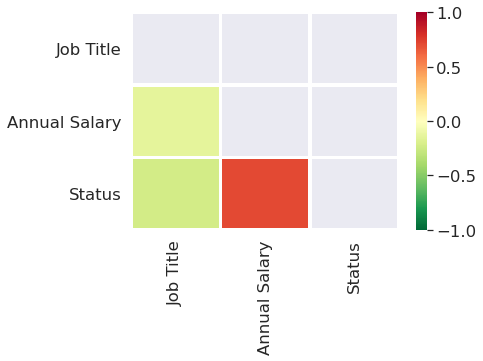
\includegraphics[width=0.7\textwidth]{figures/san_francisco_rankingfacts1.png}
\caption{Heatmap showing attribute correlations for the San Francisco dataset.}
\label{fig:san_francisco_rankingfacts1}
\end{figure}

Because of the lack of attributes, we could only use \textit{Job Title}, \textit{Status}, and \textit{Annual Salary} as ranking parameters, all with a weight of 1 as done in the Chicago case and by following the examples provided by the authors.

The following list summarizes our results by following the widget description list provided in Section~\ref{section:ranking_facts}:
\begin{itemize}
\item \textbf{Recipe} and \textbf{Ingredients}: as for the Chicago case, these widgets did not provide us any particularly useful information. For the sake of completeness, we just report that the importance of each attribute used for the ranking is effectively equal to 1.
\item \textbf{Stability}: our ranking resulted to be unstable both at top-10 (stability at 0.25) and overall (stability at 0.0). The score distribution is displayed in Figure~\ref{fig:san_francisco_rankingfacts2}.

\begin{figure}[t!]
\centering
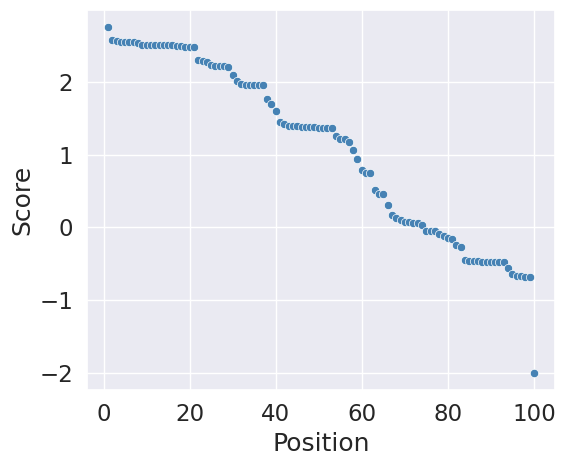
\includegraphics[width=0.7\textwidth]{figures/san_francisco_rankingfacts2.png}
\caption{Score distribution of the ranking for the San Francisco dataset.}
\label{fig:san_francisco_rankingfacts2}
\end{figure}

\item \textbf{Fairness}: recalling the fact that, for the statistical measures adopted, a ranking is considered unfair when the \(p\)-value of the corresponding test falls below 0.05, we will now recapitulate our fairness results:
\begin{itemize}
\item \textbf{FA*IR}: the ranking resulted to be \textit{fair for males}, with an approximate \(p\)-value of 0.99, and \textit{unfair for females}, with an approximate \(p\)-value of 0.01.
\item \textbf{Proportion}: the ranking resulted to be \textit{fair for males}, with an approximate \(p\)-value of 0.99, and \textit{unfair for females}, with an approximate \(p\)-value of 0.01.
\item \textbf{Pairwise}: the ranking resulted to be \textit{fair for males}, with an approximate \(p\)-value of 1.0, and \textit{unfair for females}, with an approximate \(p\)-value of 0.0.
\end{itemize}
The results seem to be oriented towards a biased dataset in favor of men, in contrast with the generally fair outcomes of the other tools.
\item \textbf{Diversity}: Figure~\ref{fig:san_francisco_rankingfacts3} shows the predominancy of the male group over the female one, especially in the top-10 of the ranking, highlighting again a problem of gender representation.

\begin{figure}[t!]
\centering
\begin{minipage}{0.45\textwidth}
\centering
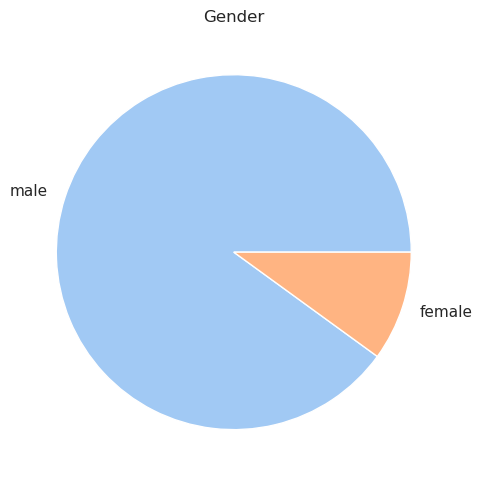
\includegraphics[width=\textwidth]{figures/san_francisco_rankingfacts3a.png}
\caption*{(a)}
\end{minipage}
\begin{minipage}{0.45\textwidth}
\centering
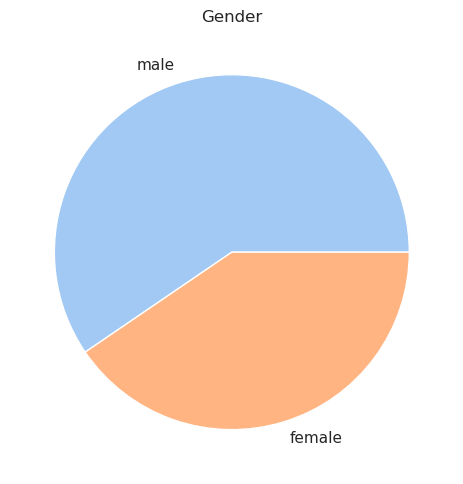
\includegraphics[width=\textwidth]{figures/san_francisco_rankingfacts3b.png}
\caption*{(b)}
\end{minipage}
\caption{\textrm{Gender} diversity widget for the top-10 (a) and overall (b) rankings of the San Francisco dataset.}
\label{fig:san_francisco_rankingfacts3}
\end{figure}

\end{itemize}


\section{Other Design Choices}
The aim of this section is to document in a technical way some experiments made on the datasets previously analyzed -- Chicago and San Francisco -- in which different design decisions were taken. It is worth to emphasize once more the importance of human choices behind computer systems, in particular when dealing with sensitive concepts such as fairness, and we believe that by looking at the impact of other design decisions we can get a broader perspective on how the tools should be used.
Because of the technical nature of this chapter, the socio-ethical impact of these choices, as well as the impact of other ones not mentioned in this section, will not be discussed here but in Section~\ref{section:XYZ}.


\subsection{Part-Time Employees Removal}
One of the first design choices we had to deal with was concerning part-time employees. The Glassdooor report \cite{chamberlain2017analyze} indeed recommends to only include full-time employees in the gender pay gap analysis (or in case of equal amounts of full-time and part-time employees to conduct two separate analyses) because of the big differences between full-time and part-time workers in the labor market. We initially decided to exclude part-time employees from the datasets, by removing their tuples and subsequently also the \textit{Status} attribute. This choice resulted to be penalizing in both our cases for different reasons:
\begin{itemize}
\item \textbf{Chicago}: for the preprocessed dataset, the number of male employees decreased from 16,146 to 15,880 (\(-\)1.65\%), while the number of female employees decreased from 4,163 to 3,790 (\(-\)8.96\%). Even though the reduction in the number of tuples is not excessive, most of the records removed are related to women, already underrepresented when compared to the number of men.
\item \textbf{San Francisco}: for the preprocessed dataset, the number of male employees decreased from 13,688 to 9,082 (\(-\)33.65\%), while the number of female employees decreased from 9,308 to 4,696 (\(-\)49.55\%). Even if the number of male and female employees removed is similar, we found the removal of 9,308 tuples from the dataset to have too much impact on the dataset itself.
\end{itemize}
Furthermore, it is important to note that the Glassdoor report is meant to be a guide for HR practitioners in analyzing the internal gender gap of a company, while we are performing our analysis not on a company but on public employees of different sectors. Lastly, the removal of the \textit{Status} variable furtherly penalizes datasets already characterized by a low number of attributes, making it more difficult to get concrete results from the tools. Because of these reasons, we decided to include again part-time employees in the datasets and to proceed in our analysis as discussed before.


\subsection{FAIR-DB: Discretization Using More Bins}
For both the Chicago and the San Francisco datasets, we decided to conduct a FAIR-DB analysis using more than just 2 bins. Therefore, we split the \textit{Annual Salary} values in 8 different interval levels (the K specification is implied): 0--39, 40--59, 60--79, 80--99, 100--119, 120--139, 140+.

We will now briefly summarize our results, without going too much into the details of the algorithm but describing the most relevant differences in comparison with the 2-bin analysis.

\begin{itemize}
\item \textbf{Chicago}: the preprocessed dataset is the same used for the 2-bin analysis, with 20,309 tuples of which 16,146 males and 4,163 females. The histogram of Figure~\ref{fig:chicago_8bins_fair-db1} shows the distribution of the annual salary of employees over their \textit{Gender} attribute. As we can notice, most women are concentrated in the 80--99 bin, which is the most numerous overall, but the proportion between men and women in lower bins is unbalanced: more than 50\% of the employees in the 0--39 bin are females, even though women represent about \(\frac{1}{5}\) of the population of the dataset.

\begin{figure}[t!]
\centering
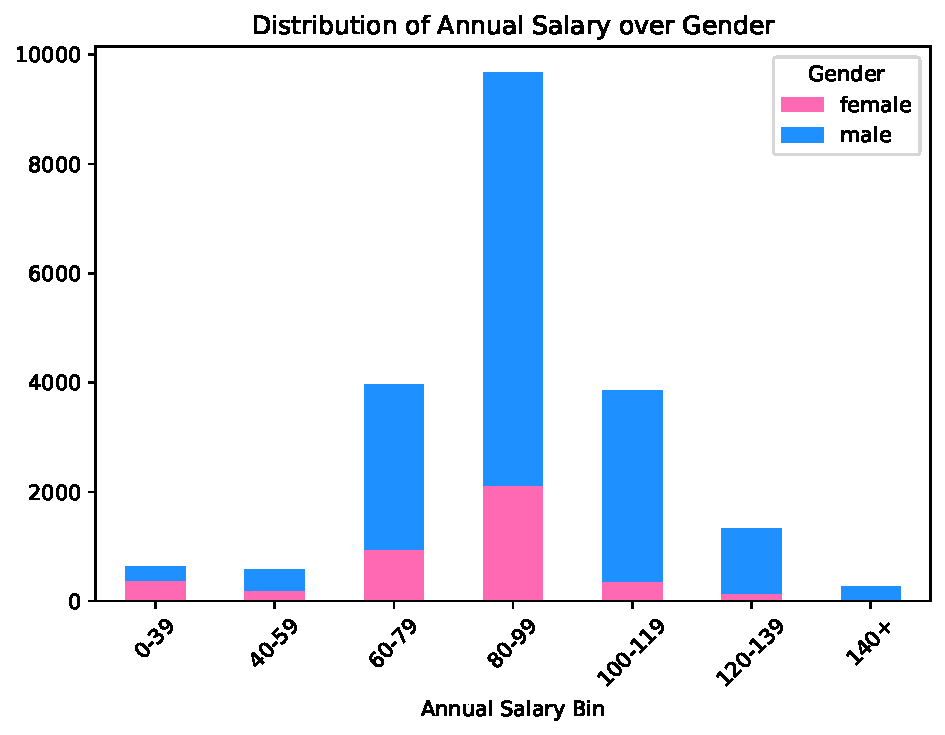
\includegraphics[width=0.75\textwidth]{figures/chicago_annual_salary_over_gender.pdf}
\caption{Distribution of the \textrm{Annual Salary} values for the Chicago dataset (8 bins).}
\label{fig:chicago_8bins_fair-db1}
\end{figure}

Since the dataset is the same as that used for the 2-bin analysis, we ran the \textit{ACFD Discovery} algorithm keeping the same parameter values: \textit{maximum~antecedent~size}~=~2, \textit{minimum~confidence}~=~0.8, and \textit{minimum~support}~=~100. The algorithm generated 759 dependencies, and the number shrinked to 193 when we filtered the results keeping only the rules containing the target attribute and its value. The automatic filtering operations performed by FAIR-DB further reduced this number from 193 to 64.

We decided to keep \textit{minimum~difference}~=~0.02 during the ACFD selection phase, in order to be able to compare the results of the two analyses and evaluate the impact of the different discretization processes performed. The first automatic selection resulted in a reduction in the number of dependencies from 64 to 28. The subsequent ACFD completion and further selection generated 172 dependencies (including the original 28), 66 of which have a difference above the threshold.

Lastly, we applied the same criterion used in the previous cases for manually choosing the rules (target attribute in the RHS). Unfortunately, we only got \(N\) = 2 out of 66 dependencies. The chosen ACFDs, together with the final scores, are displayed in Figure~\ref{fig:chicago_8bins_fair-db2}.

\begin{figure}[t!]
\centering
\noindent\rule{\linewidth}{0.4pt}\par
%\resizebox{\linewidth}{!}{%
\scalebox{.9}{\BVerbatimInput{figures/chicago_8bins_fair-db2.txt}}
\noindent\rule{\linewidth}{0.4pt}
\caption{Final selected rules and scores for the Chicago dataset (8 bins).}
\label{fig:chicago_8bins_fair-db2}
\end{figure}

As we can see, both rules refer to the ADMINISTRATIVE ASST II job title, and they suggest a discriminatory behavior in favor of women, who seem to be more paid for this specific role (even though the support of 0.00 indicates a really low percentage of tuples involved). This situation did not show up in the 2-bin analysis, because even if apparently there is a gap between salaries of men and women, all the incomes fall below the threshold of \$90K, and therefore no dependencies could have been generated. On the other side, the discriminatory behaviors detected in the 2-bin analysis, related to the AVIATION and OEMC departments, and to female employees paid on a hourly basis, were not detected here, presumibly because the annual salary values reside all in the 80--99 bin.
\item \textbf{San Francisco}: the preprocessed dataset is the same used for the 2-bin analysis, with 22,996 tuples of which 13,688 males and 9,308 females. The histogram of Figure~\ref{fig:san_francisco_8bins_fair-db1} shows the distribution of the annual salary of employees over their \textit{Gender} attribute. We can see that the ratio of the number of men to women tends to increase: in lower bins there is a balanced proportion of male and female employees, while for higher-paying jobs men are much more numerous than women.

\begin{figure}[t!]
\centering
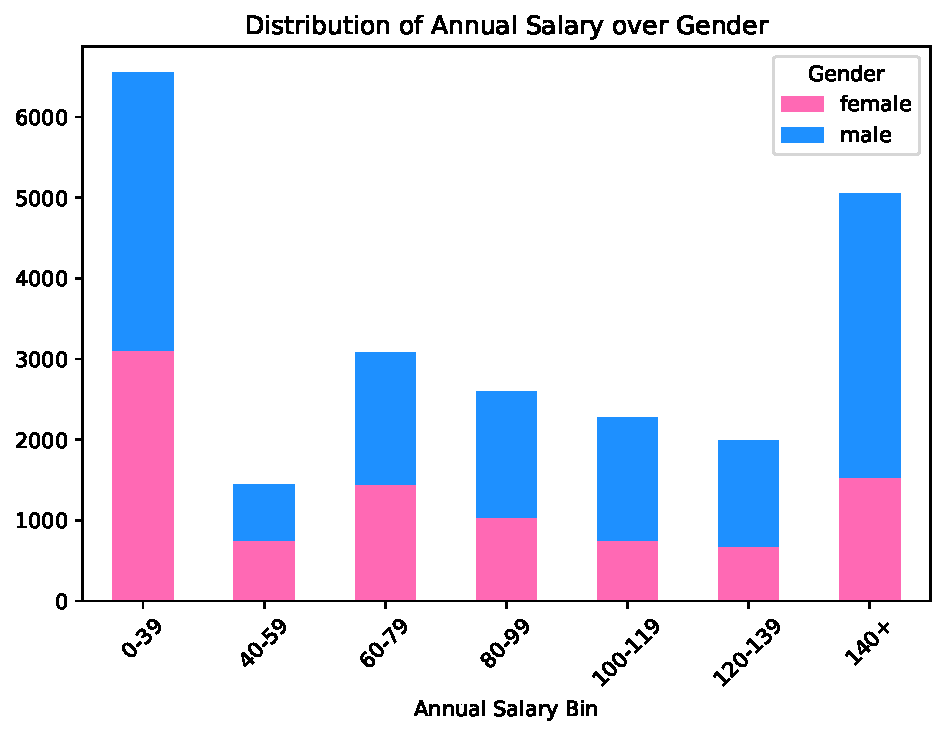
\includegraphics[width=0.75\textwidth]{figures/san_francisco_annual_salary_over_gender.pdf}
\caption{Distribution of the \textrm{Annual Salary} values for the San Francisco dataset (8 bins).}
\label{fig:san_francisco_8bins_fair-db1}
\end{figure}

Again, we kept \textit{maximum~antecedent~size}~=~2, \textit{minimum~confidence}~=~0.8, and \textit{minimum~support}~=~100 for \textit{ACFD Discovery}. The algorithm generated 465 dependencies, and the number shrinked to 144 when we filtered the results keeping only the rules containing the target attribute and its value. The automatic filtering operations performed by FAIR-DB further reduced this number from 144 to 40.

By keeping \textit{minimum~difference}~=~0.02, the first automatic ACFD selection resulted in a reduction in the number of dependencies from 40 to 20. The subsequent ACFD completion and further selection generated 154 dependencies (including the original 20), 62 of which with a difference above the threshold.

At the end, we got \(N\) = 6 out of 62 dependencies in the ACFD user selection phase. The chosen ACFDs, together with the final scores, are displayed in Figure~\ref{fig:san_francisco_8bins_fair-db2}.

\begin{figure}[t!]
\centering
\noindent\rule{\linewidth}{0.4pt}\par
%\resizebox{\linewidth}{!}{%
\scalebox{.9}{\BVerbatimInput{figures/san_francisco_8bins_fair-db2.txt}}
\noindent\rule{\linewidth}{0.4pt}
\caption{Final selected rules and scores for the San Francisco dataset (8 bins).}
\label{fig:san_francisco_8bins_fair-db2}
\end{figure}

The 6 final rules obtained are quite peculiar because they refer just to 2 different job titles. For what concerns junior clerks, men seem to be less paid then women. For the Engineer job title instead, women tend to earn less, and their incomes vary widely, since they fall within 3 different interval levels (0--39, 40--59, 120--139), while male engineers are paid more than \$140K. As for the Chicago case, the 2-bin analysis could not detect any of these discriminatory behaviors, because in the former case the salary values are all lower than the threshold, while in the latter case the presence of female engineers earning between \$120K and \$139K ``balanced'' the gap, eluding the algorithm. For the same reasons, none of the discriminatory behaviors detected through the 2-bin analysis has been observed here.
\end{itemize} 


\subsection{FAIR-DB: Choice of Different Dependencies}
As already specified, the ACFD user selection phase of the FAIR-DB framework is a delicate step, because the user needs to manually select \(N\) among all the dependencies for the subsequent scoring and calculation of the metrics. In Section~\ref{section:chicago_fair-db} we clarified the reasons why we decided to always keep rules in which the target attribute is in the RHS. However, during our first experiments, we tried to select all the dependencies, in order to check the impact of the user choices on the final results. The experiments were conducted on the same preprocessed datasets, and using the same parameter values; the only difference is indeed the selection of every rule instead of just some of them. The following results refer to the 8-bin analysis:
\begin{itemize}
\item \textbf{Chicago}: by selecting all 66 dependencies, we got a cumulative support of 0.856, meaning that 85.6\% of the dataset is ``problematic'' (17,384 tuples out of 20,309). The difference mean value is 0.153, while the gender difference mean is equal to 0.071. The measures have different values because for most rules (of which all with the target attribute in the LHS) the p-Difference is NaN, while the difference is not.
\item \textbf{San Francisco}: by selecting all 62 dependencies, we got a cumulative support of 0.925, meaning that 92.5\% of the dataset is ``problematic'' (21,279 tuples out of 22,996). The difference mean value is 0.153, while the gender difference mean is equal to 0.003.
\end{itemize}
We can conclude that the user choices in this phase strongly impact the final outcomes, since a dataset results to be fair or not depending on the selected rules. In both our cases, the gap is huge: for Chicago the percentage of ``problematic'' tuples shifted from 0.4\% (as we can see from the cumulative support in Figure~\ref{fig:chicago_8bins_fair-db2}) to 85.6\%, while for San Francisco the same percentage shifted from 1\% (Figure~\ref{fig:san_francisco_8bins_fair-db2}) to 92.5\%.


\subsection{Grouping of Job Titles}
Another recommendation from the Glassdoor report \cite{chamberlain2017analyze} is the one of grouping together similar job titles, because having too many unique roles with just a few workers in each could make the analysis less reliable. Therefore, we decided to test our tools on a slightly different version of the Chicago dataset, in which the data preprocessing phase consists of one more step: a \textbf{generalization} of the \textit{Job Title} values. We opted for the Chicago dataset instead of the San Francisco one mostly because a certain degree of precision is required in classifying job titles, and since the classification has to be performed manually we preferred to deal with 35 distinct \textit{Job Title} values rather than 81. In order to group job titles in a sensible way, we relied on a document published by the Equality Commission for Northern Ireland in 2013 \cite{equality2013index}. Even though the document refers to Northern Ireland, it provides an exhaustive list of thousands of different job titles, together with a few introductory sections on how to use the index, and we found useful to rely on these guidelines in grouping the job titles of our dataset. The document, based on the Standard Occupational Classification 2010 (SOC2010) -- a common classification of occupational information for the UK -- distinguishes between 9 different major groups:
\begin{itemize}
\item[1.] Managers and senior officials
\item[2.] Professional occupations
\item[3.] Associate professional and technical occupations
\item[4.] Administrative and secretarial occupations
\item[5.] Skilled trades occupations
\item[6.] Personal service occupations
\item[7.] Sales and customer service occupations
\item[8.] Process, plant and machine operatives
\item[9.] Elementary occupations
\end{itemize}
The index then provides correspondencies between each job title and the major group to which it belongs. Figure~\ref{fig:encodings} shows the correspondencies between our job titles and the related major groups, together with the index entries of reference. It is worth to mention that we decided to overwrite the previous \textit{Job Title} values with the corresponding major group numbers, transforming the categorical attribute into numeric.

\begin{figure}[t!]
\centering
\noindent\rule{\linewidth}{0.4pt}\par
%\resizebox{\linewidth}{!}{%
\scalebox{.9}{\BVerbatimInput{figures/encodings.txt}}
\noindent\rule{\linewidth}{0.4pt}
\caption{Correspondencies between \textrm{Job Title} values for the Chicago dataset and related major groups, together with index entries of reference.}
\label{fig:encodings}
\end{figure}

We will now provide the results of the analysis of the modified dataset:
\begin{itemize}
\item \textbf{The ``Glassdoor Method''}: we detected a bigger gap (in favor of men) in the average salaries of male and female employees for a few job title values. In particular, the most significant differences are related to job title 2 (professional occupations), in which the average income for men is \$102,539.79 while for women is \$73,827.52, and job title 6 (personal service occupations), in which the average income for men is \$75,868.14 while for women is \$42,134.53.

These differences slightly impacted the \textit{Male} coefficient of the ``adjusted pay gap'', bringing its value from 0.004 (standard Chicago dataset) to 0.034, meaning that men on average earn 3,4\% more than women. The result, however, remains not statistically significant, and we cannot infer the presence of a systematic gender pay gap.
\item \textbf{FAIR-DB}: we conducted a 2-bin analysis with the usual \$90K threshold, keeping the same parameter values used in previous scenarios and applying the same criterion for the manual selection of the rules (target attribute in the RHS).

\textit{ACFD Discovery} detected 547 dependencies, whose number shrinked to 122 when we filtered the results keeping only the rules containing the target attribute and its value. The automatic filtering operations performed by FAIR-DB further reduced this number from 122 to 38.

The first automatic ACFD selection resulted in a reduction in the number of dependencies from 38 to 18, while the subsequent ACFD completion and further selection generated 68 dependencies (including the original 18), 31 of which with a difference above the threshold.

At the end, we got \(N\) = 10 out of 31 dependencies in the ACFD user selection phase. The chosen ACFDs, together with the final scores, are displayed in Figure~\ref{fig:chicago_grouped_fair-db}.

\begin{figure}[t!]
\centering
\noindent\rule{\linewidth}{0.4pt}\par
%\resizebox{\linewidth}{!}{%
\scalebox{.9}{\BVerbatimInput{figures/chicago_grouped_fair-db.txt}}
\noindent\rule{\linewidth}{0.4pt}
\caption{Final selected rules and scores for the Chicago dataset with grouped job titles (2 bins).}
\label{fig:chicago_grouped_fair-db}
\end{figure}

As we can see, the algorithm detected the same dependencies of the standard Chicago case, with the introduction of 4 more rules, 2 of which related to job title 2 (professional occupations), already observed as problematic in the ``Glassdoor Method'' analysis. The other dependencies, not related to each other, suggest that females employed in job title 8 (process, plant and machine operatives) tend to earn less than \$90K, and the same holds for males employed in job title 4 (administrative and secretarial occupations).

The cumulative support is obviously higher than the one of the standard Chicago scenario, because the same rules have been detected, together with 4 more dependencies involving other tuples. The increment however is not significantly impactful on the results (from 11.4\% to 12\% of the dataset marked as ``problematic'').
\item \textbf{Ranking Facts}: the generalization process performed on the \textit{Job Title} attribute did not have an impact on the number of tuples of the dataset, and therefore we still had to rely on the notebook version. The impact on the heatmap was also minimal, and we avoid to report it here because no new significant correlations between attributes were highlighted. We used the same attributes and weights of the standard Chicago case for the ranking (\textit{Job Title}, \textit{Department}, \textit{Status}, \textit{Salary or Hourly}, \textit{Annual Salary}), and the results are summarized as follows:
\begin{itemize}
\item \textbf{Recipe} and \textbf{Ingredients}: no particularly useful information from these widgets. As done before, we just report that the importance of each attribute used for the ranking is effectively equal to 1.
\item \textbf{Stability}: as for the standard Chicago case, the ranking resulted to be stable at top-10 (stability at 0.28) but unstable overall (stability at 0.0).
\item \textbf{Fairness}: the statistical measures adopted provided us with the following results:
\begin{itemize}
\item \textbf{FA*IR}: the ranking resulted to be \textit{fair for males}, with an approximate \(p\)-value of 0.9, and \textit{fair for females}, with an approximate \(p\)-value of 0.1. The grouping operation resulted, for this metric, in a change in the female-related outcome in comparison with the standard Chicago case.
\item \textbf{Proportion}: the ranking resulted to be \textit{fair for males}, with an approximate \(p\)-value of 0.89, and \textit{fair for females}, with an approximate \(p\)-value of 0.18. Both values decreased in comparison with the standard Chicago case (respectively 0.97 and 0.35), but the related outcomes remained the same.
\item \textbf{Pairwise}: the ranking resulted to be \textit{fair for males}, with an approximate \(p\)-value of 1.0, and \textit{unfair for females}, with an approximate \(p\)-value of 0.0. The grouping operation resulted, for this metric, in a change in the female-related outcome in comparison with the standard Chicago case.
\end{itemize}
Similarly to the standard Chicago case, the results seem to be oriented towards a fair dataset, even though the pairwise measure reported the presence of bias in favor of men.
\item \textbf{Diversity}: Figure~\ref{fig:chicago_grouped_rankingfacts} shows the \textit{Gender} diversity widget for the top-10 and overall rankings. As we can notice, even though there is still a predominancy of the male group over the female one, in the top-10 ranking women seem to be slightly more represented than in the standard Chicago case, in which the whole chart was occupied by men.

\begin{figure}[t!]
\centering
\begin{minipage}{0.45\textwidth}
\centering
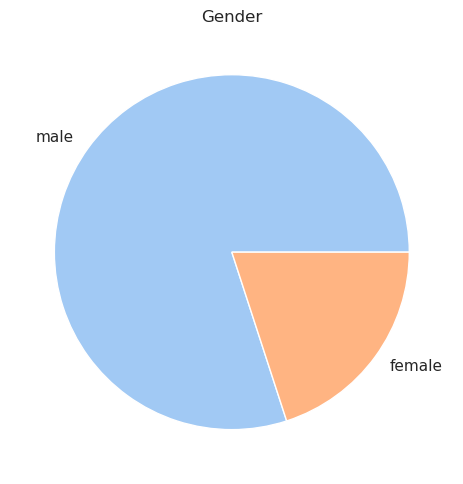
\includegraphics[width=\textwidth]{figures/chicago_grouped_rankingfacts1a.png}
\caption*{(a)}
\end{minipage}
\begin{minipage}{0.45\textwidth}
\centering
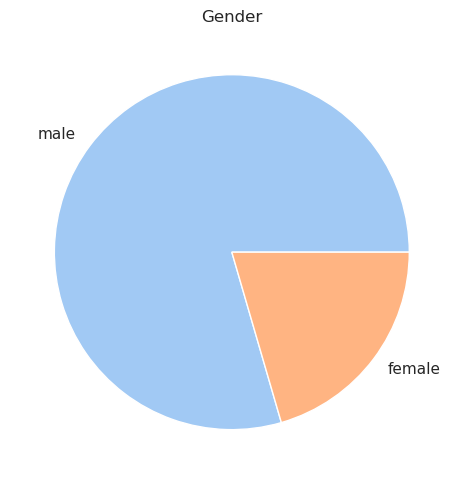
\includegraphics[width=\textwidth]{figures/chicago_grouped_rankingfacts1b.png}
\caption*{(b)}
\end{minipage}
\caption{\textrm{Gender} diversity widget for the top-10 (a) and overall (b) rankings of the Chicago dataset with grouped job titles.}
\label{fig:chicago_grouped_rankingfacts}
\end{figure}

\end{itemize}
\end{itemize}


\subsection{Voluntary Introduction of Bias}
In order to test the tools on a clearly biased dataset, we decided to modify the Chicago one by halving the \textit{Annual Salary} value of female employees. This kind of operations generates a \textbf{synthetic dataset}, that is, a dataset containing fake data, not reflecting the real world in which we live. In other words, from the tools perspective, modifying the dataset means modifying the reality, and even if this consideration is applicable to every operation performed on data, in this specific context the original dataset undergoes such an impactful change that it becomes, as mentioned before, synthetic. Recalling the concepts discussed in Chapter~\ref{chapter2}, we can say we voluntarily introduced some technical bias with the aim of simulating the presence of preexisting bias in the society. Our main reason for generating a synthetic dataset is, in fact, to test the tools on data that we know for sure to be discriminatory.

Apart for the change in wage values of female employees, the preprocessed dataset is the same used in the standard Chicago case, with 20,309 tuples of which 16,146 males and 4,163 females. We will now provide the results of the analysis of the modified dataset:
\begin{itemize}
\item \textbf{The ``Glassdoor Method''}: for the sake of brevity, we avoid reporting summary table, pivot table, and average salaries for men and women, since the information provided by them reflects the dramatic modification on the income of female employees.

\begin{figure}[t!]
\centering
\noindent\rule{\linewidth}{0.4pt}\par
%\resizebox{\linewidth}{!}{%
\scalebox{.9}{\BVerbatimInput{figures/chicago_biased_glassdoor.txt}}
\noindent\rule{\linewidth}{0.4pt}
\caption{Regression results for the biased Chicago dataset.}
\label{fig:chicago_biased_glassdoor}
\end{figure}

Figure~\ref{fig:chicago_biased_glassdoor} shows instead our results: a coefficient of 0.935 on the male-female dummy variable means there is approximately 93.5\% ``unadjusted'' pay gap (therefore, men on average earn 93.5\% more than women), and adding to the model all of the controls available in the data the coefficient value shrinks to 69.7\%, remaining statistically significant. As we expected, the final outcome is significantly different from the standard Chicago case, and there is clear evidence of a systematic gender pay gap even on an ``adjusted'' basis.
\item \textbf{FAIR-DB}: we conducted a 2-bin analysis with the usual \$90K threshold, keeping the same parameter values used in previous scenarios and applying the same criterion for the manual selection of the rules (target attribute in the RHS).

\textit{ACFD Discovery} detected 785 dependencies, whose number shrinked to 161 when we filtered the results keeping only the rules containing the target attribute and its value. The automatic filtering operations performed by FAIR-DB further reduced this number from 161 to 35.

The first automatic ACFD selection resulted in a reduction in the number of dependencies from 35 to 20, while the subsequent ACFD completion and further selection generated 79 dependencies (including the original 20), 39 of which with a difference above the threshold.

At the end, we got \(N\) = 32 out of 39 dependencies in the ACFD user selection phase. The chosen ACFDs, together with the final scores, are displayed in Figure~\ref{fig:chicago_biased_fair-db}. For readability reasons, the indication of the number of tuples concerned by the rules (13,311) and the total number of tuples (20,309) is not included in the image.

\begin{figure}[t!]
\centering
\noindent\rule{\linewidth}{0.4pt}\par
%\resizebox{\linewidth}{!}{%
\scalebox{.9}{\BVerbatimInput{figures/chicago_biased_fair-db1a.txt}}
\phantomcaption
\end{figure}
\begin{figure}[t!]
\ContinuedFloat
\centering
%\resizebox{\linewidth}{!}{%
\scalebox{.9}{\BVerbatimInput{figures/chicago_biased_fair-db1b.txt}}
\noindent\rule{\linewidth}{0.4pt}
\caption{Final selected rules and scores for the biased Chicago dataset (2 bins).}
\label{fig:chicago_biased_fair-db}
\end{figure}

The algorithm detected pairs of dependencies related to 14 distinct \textit{Job Title} values (out of 35), for which female employees earn less than \$90K while male employees earn more than \$90K. All of these are job titles in which the standard income is higher than the threshold, and this is the reason why the voluntary introduction of bias had an impact on the results. For the 21 other \textit{Job Title} values, indeed, the average salary is lower than \$90K even for males, and the gender pay gap could not be observed. Decreasing the threshold value would be an option to include more job titles in the results, but then the opposite risk may occur: jobs for which the average income would be higher than the threshold even for females would not be detected. It is worth to mention the presence of rules 14 and 11, concerning the DAIS department, which has to be related one to one to a job title for which the average wage is higher than \$90K, and it is important to highlight the presence of rules 3 and 0, which ``generalize'' the gender pay gap problem specifying that in general, regardless of the job title, women always earn less than \$90K while most men do not.

For what concerns the metrics, we can notice that for all the female-related rules (and for most of the others) the confidence parameter is equal to 1, meaning that these dependencies hold for all the tuples with the attribute values specified in the LHS. The cumulative support is high (65.5\% of the dataset is ``problematic'') because, even if most of the rules are related to specific job titles, rules 3 and 0 involve a significant amount of tuples. We can finally notice high values for the difference measure for all the female-related rules, indicating a high ``unethical'' level towards women.
\item \textbf{Ranking Facts}: the voluntary introduction of bias did not have an impact on the number of tuples of the dataset, and therefore we still had to rely on the notebook version. The impact on the heatmap was also minimal, and we avoid to report it here because no new significant correlations between attributes were highlighted. We used the same attributes and weights of the standard Chicago case for the ranking (\textit{Job Title}, \textit{Department}, \textit{Status}, \textit{Salary or Hourly}, \textit{Annual Salary}), and the results are summarized as follows:
\begin{itemize}
\item \textbf{Recipe} and \textbf{Ingredients}: no particularly useful information from these widgets. As done before, we just report that the importance of each attribute used for the ranking is effectively equal to 1.
\item \textbf{Stability}: as for the standard Chicago case, the ranking resulted to be stable at top-10 (stability at 0.3) but unstable overall (stability at 0.0).
\item \textbf{Fairness}: the statistical measures adopted provided us with the following results:
\begin{itemize}
\item \textbf{FA*IR}: the ranking resulted to be \textit{fair for males}, with an approximate \(p\)-value of 1.0, and \textit{unfair for females}, with an approximate \(p\)-value of 0.0. Even though both values changed in comparison with the standard Chicago case (respectively 0.84 and 0.16), the related outcomes remained the same.
\item \textbf{Proportion}: the ranking resulted to be \textit{fair for males}, with an approximate \(p\)-value of 1.0, and \textit{unfair for females}, with an approximate \(p\)-value of 0.0. The voluntary introduction of bias resulted, for this metric, in a change in the female-related outcome in comparison with the standard Chicago case.
\item \textbf{Pairwise}: the ranking resulted to be \textit{fair for males}, with an approximate \(p\)-value of 1.0, and \textit{unfair for females}, with an approximate \(p\)-value of 0.0. The voluntary introduction of bias resulted, for this metric, in a change in the female-related outcome in comparison with the standard Chicago case.
\end{itemize}
As we expected, the results seem to be oriented towards an unfair dataset, in which women are discriminated against.
\item \textbf{Diversity}: Figure~\ref{fig:chicago_biased_rankingfacts} shows the \textit{Gender} diversity widget for the top-10 and overall rankings. As we expected, the charts look identical to the standard Chicago case, with the top-10 ranking monopolized by men.

\begin{figure}[t!]
\centering
\begin{minipage}{0.45\textwidth}
\centering
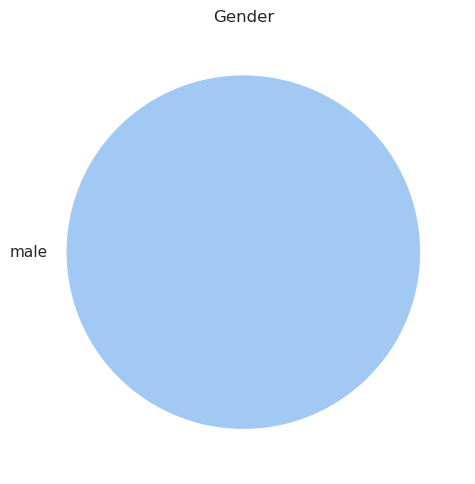
\includegraphics[width=\textwidth]{figures/chicago_biased_rankingfacts1a.png}
\caption*{(a)}
\end{minipage}
\begin{minipage}{0.45\textwidth}
\centering
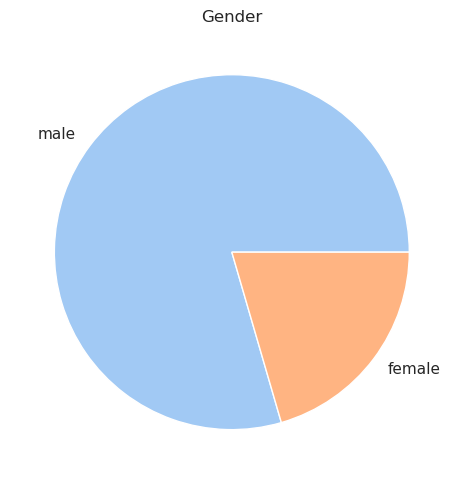
\includegraphics[width=\textwidth]{figures/chicago_biased_rankingfacts1b.png}
\caption*{(b)}
\end{minipage}
\caption{\textrm{Gender} diversity widget for the top-10 (a) and overall (b) rankings of the biased Chicago dataset.}
\label{fig:chicago_biased_rankingfacts}
\end{figure}

\end{itemize}
\end{itemize}
